\chapter{Arithmetic}
    We begin by introducing the concept of \textit{number}. We use
    intuition by using these to count, discussing the
    \textit{natural numbers}, or positive integers, and end with an
    exposition to \textit{real} numbers.
    \section{Sets}
        Before we discuss numbers, it is good to familiarize oneself
        with some of the basic objects that arise in mathematics. The
        most basic of which are called \textit{sets}.
        \begin{fdefinition}{Sets}{Sets}
            A set is a collection of objects, none of which
            is the set itself.
        \end{fdefinition}
        The requirement that a set cannot contain itself is to avoid
        logical paradoxes, such as the one discovered by Bertrand
        Russell in 1901. The objects contained in a set are called
        the elements of that set. We use the following notation to
        denote which elements belong to a set:
        \begin{fnotation}{Set Notation}{Element_Notation}
            If $A$ is a set and $x$ is an element of $A$, then we
            write $x\in{A}$. If $x$ is not an element of $A$, then
            we write $x\notin{A}$.
        \end{fnotation}
        \begin{lexample}{Using Set Notation}{Using_Set_Notation}
            Let $A$ be the set of all days of the week. Then
            $\textrm{Saturday}\in{A}$. This reads
            \textit{Saturday is an element of the set} $A$. Since
            $A$ is the set of all days of the week, and since
            Saturday is one of the days of the week, it is true that
            Saturday is an element of $A$. Hence, we are justified
            in writing $\textrm{Saturday}\in{A}$.
        \end{lexample}
        Sets are usually described by one of two methods. The first
        way is to list out all of the elements, separated by commas,
        and enclosing them in braces.
        \begin{lexample}{Elementary Examples of Sets}
                        {Elementary_Examples_of_Sets}
            When a set isn't too big it is easiest to describe it by
            listing out all of the elements, enclosing them in
            braces. For example:
            \par
            \begin{subequations}
                \begin{minipage}{0.49\textwidth}
                    \centering
                    \begin{equation}
                        A=\{\,1,\,2,\,3\,\}
                    \end{equation}
                \end{minipage}
                \hfill
                \begin{minipage}{0.49\textwidth}
                    \centering
                    \begin{equation}
                        B=\{\,a,\,b,\,c\,\}
                    \end{equation}
                \end{minipage}
            \end{subequations}
            \par\vspace{2.5ex}
            Using our notation (Notation~\ref{not:Element_Notation})
            we see that $1\in{A}$, since 1 is an element of the set $A$,
            but $4\notin{A}$ since 4 is not contained in $A$.
            Similarly, $a\in{B}$ but $d\notin{B}$.
        \end{lexample}
        When a set has infinitely many elements, but the elements can
        be listed in a certain pattern, we use ellipses to indicate
        the pattern goes on. For example, we can write the set of all
        \textit{natural numbers}, or counting numbers, as:
        \begin{equation}
            \mathbb{N}=\{\,1,\,2,\,3,\,\hdots\,\}
        \end{equation}
        The symbol $\mathbb{N}$ stands for \textit{natural}. It is
        very common to write the set of all natural numbers using this
        symbol. Ellipses can be used to describe other sets:
        \par
        \begin{subequations}
            \begin{minipage}{0.49\textwidth}
                \centering
                \begin{equation}
                    \mathbb{N}_{e}=\{\,2,\,4,\,6,\,8,\,\hdots\,\}
                \end{equation}
            \end{minipage}
            \hfill
            \begin{minipage}{0.49\textwidth}
                \centering
                \begin{equation}
                    \mathbb{N}_{o}=\{\,1,\,3,\,5,\,7,\,\hdots\,\}
                \end{equation}
            \end{minipage}
        \end{subequations}
        \par\vspace{2.5ex}
        Which denote the set of all even and odd positive integers,
        respectively. As a reminder, an even integer is an integer that
        is divisible by 2, and an odd integer is an integer that is not
        divisible by 2. All even integers can be written as $n=2k$,
        where $k$ is also some integer. Similarly, every odd integer can
        be written as $n=2k+1$, where $k$ is some integer. This brings
        us to the second way to describe a set: Set-Builder notation.
        We can describe $\mathbb{N}_{e}$ and $\mathbb{N}_{o}$ by writing:
        \par
        \begin{subequations}
            \begin{minipage}{0.49\textwidth}
                \centering
                \begin{equation}
                    \label{eqn:Even_Nat_Def}%
                    \mathbb{N}_{e}=\{\;2k:k\in\mathbb{N}\;\}
                \end{equation}
            \end{minipage}
            \hfill
            \begin{minipage}{0.49\textwidth}
                \centering
                \begin{equation}
                    \label{eqn:Odd_Nat_Def}%
                    \mathbb{N}_{o}=\{\;2k+1:k\in\mathbb{N}\;\}
                \end{equation}
            \end{minipage}
        \end{subequations}
        \par\vspace{2.5ex}
        Eqn.~\ref{eqn:Even_Nat_Def} says that $\mathbb{N}_{e}$ is the
        set of all positive multiples of 2, which is precisely the
        definition of an even natural number. Similarly,
        Eqn.~\ref{eqn:Odd_Nat_Def} says that $\mathbb{N}_{o}$ is the set
        of all positive multiples of 2, plus 1. Again, this is the
        definition of an odd number. Set-Builder notation often makes
        it possible to describe very large sets in a very compact manner.
        We can even use plain English:
        \begin{equation}
            \mathbb{N}=\{\;n:n\textrm{ is a positive integer}\;\}
        \end{equation}
        This is the set of all $n$ such that $n$ is a positive integer.
        \begin{lexample}{}{}
            As another example, we could write
            the set of all days of the week as:
            \begin{equation}
                \{\;x:x\textrm{ is a day of the week}\;\}
                =\{\;\textrm{Sunday, Monday, ..., Saturday}\;\}
            \end{equation}
            Both are equivalent representations of the same set. Sets
            can be abstract and may have nothing to do with numbers.
            The elements themselves need not be related to each other,
            nor need they be \textit{mathematical} in nature. Consider
            the following:
            \begin{subequations}
                \begin{minipage}{0.49\textwidth}
                    \centering
                    \begin{equation}
                        C=\{\,\textrm{Boston, Seattle}\,\}
                    \end{equation}
                \end{minipage}
                \hfill
                \begin{minipage}{0.49\textwidth}
                    \centering
                    \begin{equation}
                        O=\{\,\textrm{Atlantic, Pacific}\,\}
                    \end{equation}
                \end{minipage}
            \end{subequations}
            \par\vspace{2.5ex}
            Here, $C$ is a set containing the names of two
            cities, and $O$ is a set containing two oceans.
            We will mostly be studying sets of numbers, and
            in particular the set of \textit{real} numbers
            and their properties.
        \end{lexample}
            It is possible for two different
            sets to contain the
            same elements, and for two different
            sets to contain
            completely different elements.
            An important concept in the study of
            sets is that of \textit{subsets}. If
            $A$ and $B$ are sets and if every
            element of $A$ is also an element of $B$,
            we call $A$ a subset of $B$.
            \begin{fdefinition}{Subsets}{Subset}
                A subset of a set $B$ is a set $A$
                such that for all $x\in{A}$,
                it is true that $x\in{B}$. If $A$ is a
                subset of a set $B$, then we write
                $A\subseteq{B}$. If not, we write
                $A\not\subseteq{B}$.
            \end{fdefinition}
            \begin{figure}[H]
                \centering
                \captionsetup{type=figure}
                %--------------------------------Dependencies----------------------------------%
%   tikz                                                                       %
%-------------------------------Main Document----------------------------------%
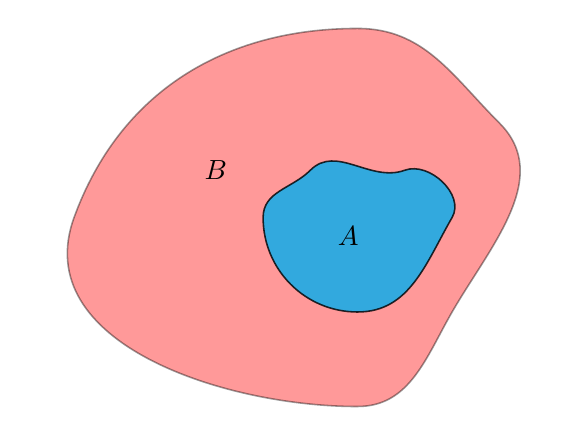
\begin{tikzpicture}[line width=0.2mm, scale=1.2]

    % Coordinates for the bigger blob.
    \coordinate (P1) at ( 0.0, -2.0);
    \coordinate (P2) at ( 1.0, -1.0);
    \coordinate (P3) at ( 1.5,  1.0);
    \coordinate (P4) at ( 0.0,  2.0);
    \coordinate (P5) at (-3.0,  0.0);

    % Coordinates for the inner blob.
    \coordinate (Q1) at ( 0.0, -1.0);
    \coordinate (Q2) at ( 1.0,  0.0);
    \coordinate (Q3) at ( 0.5,  0.5);
    \coordinate (Q4) at (-0.5,  0.5);
    \coordinate (Q5) at (-1.0,  0.0);

    % Coordindates to label things.
    \coordinate (A) at (-0.1, -0.2);
    \coordinate (B) at (-1.5,  0.5);

    % Draw the bigger blob.
    \draw[fill=red, opacity=0.4] (P1) to [out=0,    in=-120] (P2)
                                      to [out=60,   in=-45]  (P3)
                                      to [out=135,  in=0]    (P4)
                                      to [out=-180, in=70]   (P5)
                                      to [out=-110, in=-180] cycle;

    % Draw the inner blob.
    \draw[fill=cyan, opacity=0.8] (Q1) to [out=0,    in=-120]  (Q2)
                                       to [out=60,   in=20]    (Q3)
                                       to [out=-160, in=45]    (Q4)
                                       to [out=-135, in=90]    (Q5)
                                       to [out=-90,  in=180]   cycle;

    % Labels for the two blobs.
    \node at (A) {$A$};
    \node at (B) {$B$};
\end{tikzpicture}

                \caption[Visual for Subsets]
                        {Sets can often be visualized as blobs.
                         The blob $A$ is entirely contained
                         inside the blob $B$, and thus we say
                         that $A$ is a
                         \textit{subset} of $B$. Mathematically,
                         we write this
                         as $A\subseteq{B}$.}
                \label{fig:Elem_Alg_Subsets_Example}
            \end{figure}
            \begin{lexample}{}{}
                Previously, in Eqns.~\ref{eqn:Even_Nat_Def} and
                \ref{eqn:Odd_Nat_Def}, we used set-builder notation to
                define the set of positive \textit{even} integers and
                positive \textit{odd} integers. From the definitions, every
                positive even integer is a positive integer, and every
                positive odd integer is a positive integer.
                Thus, we have the following:
                \par
                \begin{subequations}
                    \begin{minipage}{0.49\textwidth}
                        \centering
                        \begin{equation}
                            \mathbb{N}_{e}\subseteq\mathbb{N}
                        \end{equation}
                    \end{minipage}
                    \hfill
                    \begin{minipage}{0.49\textwidth}
                        \centering
                        \begin{equation}
                            \mathbb{N}_{o}\subseteq\mathbb{N}
                        \end{equation}
                    \end{minipage}
                \end{subequations}
                \par\vspace{2.5ex}
                We also see that none of the elements of
                $\mathbb{N}_{e}$ are elements of $\mathbb{N}_{o}$,
                and similarly none of the elements of
                $\mathbb{N}_{e}$ are elements of $\mathbb{N}_{o}$.
                Thus, we have:
                \par
                \begin{subequations}
                    \begin{minipage}{0.49\textwidth}
                        \centering
                        \begin{equation}
                            \mathbb{N}_{e}\nsubseteq\mathbb{N}_{o}
                        \end{equation}
                    \end{minipage}
                    \hfill
                    \begin{minipage}{0.49\textwidth}
                        \centering
                        \begin{equation}
                            \mathbb{N}_{e}\nsubseteq\mathbb{N}_{o}
                        \end{equation}
                    \end{minipage}
                \end{subequations}
                \par\vspace{2.5ex}
                Moreover, $\mathbb{N}_{e}$ and $\mathbb{N}_{o}$ are
                \textit{disjoint}: They have no elements in common.
            \end{lexample}
            If we want to be rigorous we can use the notion of
            subset to define equality. Two things are equal if they
            are the exact same thing. This is slightly vague, and a
            clearer definition is needed.
            \begin{ldefinition}{Equal Sets}{Equal_Sets}
                Equal sets are sets $A$ and $B$ such that
                $A\subseteq{B}$ and $B\subseteq{A}$. If $A$ and $B$
                are equal set, then we write $A=B$.
            \end{ldefinition}
            This says that $A$ and $B$ are equal if and only if
            they have the exact same elements. Thus, this definition
            gives us our intuitive notion of equality, and is
            rigorous enough to do higher mathematics.
            \begin{theorem}
                \label{thm:Set_Is_Sub_of_Self}%
                If $A$ is a set, then $A\subseteq{A}$.
            \end{theorem}
            \begin{proof}
                If $A$ is a set, then for all $x\in{A}$ it is true that
                $x\in{A}$. Thus, $A\subseteq{A}$.
            \end{proof}
            \begin{theorem}
                If $A$ is a set, then $A=A$.
            \end{theorem}
            \begin{proof}
                By Thm.~\ref{thm:Set_Is_Sub_of_Self},
                $A\subseteq{A}$. Thus, by the definition of
                equality (Def.~\ref{def:Equal_Sets}),
                $A=A$. Therefore, etc.
            \end{proof}
            It is often useful to distinguish between subsets
            that do not contain \textit{all} of the elements of
            the given set. These are called \textit{proper subsets}.
            \begin{ldefinition}{Proper Subset}{Proper_Subset}
                A proper subset of a set $B$ is a set $A$ such that
                $A\subseteq{B}$, and $A\ne{B}$. That is, there is
                an element $b\in{B}$ such that $b\notin{A}$. We
                denote this by writing $A\subsetneq{B}$.
            \end{ldefinition}
            By examining Fig.~\ref{fig:Elem_Alg_Subsets_Example}
            we see that blob $A$ is entirely contained within blob $B$,
            and thus $A\subseteq{B}$. However, there are parts of $B$
            that are not contained in $A$, and therefore $A\ne{B}$. We can
            summarize this by saying that $A$ is a \textit{proper} subset
            of $B$, and write $A\subsetneq{B}$. We should be careful with
            notation here, since the two look very similar. $A\subseteq{B}$
            says that $A$ is a subset of $B$, and it may be possible that
            $A=B$. $A\subsetneq{B}$ says that $A$ is a subset of
            $B$, and $A\ne{B}$.
            \begin{lexample}{}{}
                Let $A$ and $B$ be sets defined as follows:
                \par
                \begin{subequations}
                    \begin{minipage}[b]{0.49\textwidth}
                        \centering
                        \begin{equation}
                            A=\{\,1,\,2,\,3,\,4,\,5\,\}
                        \end{equation}
                    \end{minipage}
                    \hfill
                    \begin{minipage}[b]{0.49\textwidth}
                        \centering
                        \begin{equation}
                            B=\{\,1,\,2,\,3,\,4,\,5,\,6,\,7,\,8\,\}
                        \end{equation}
                    \end{minipage}
                \end{subequations}
                \par\vspace{2.5ex}
                Then $A\subseteq{B}$ for every number contained
                in $A$ is contained in also $B$. However,
                $B\not\subseteq{A}$, for there are elements of $B$
                that are not in $A$. For example, $7\in{B}$ but
                $7\notin{A}$. Therefore $A$ is a
                proper subset of $B$, and we write
                $A\subsetneq{B}$. As another example, consider
                the following sets:
                \begin{subequations}
                    \begin{align}
                        C&=\{\,\textrm{Atlantic, Pacific}\,\}\\
                        D&=\{\,\textrm{Atlantic, Pacific,
                                       Arctic, Indian}\,\}
                    \end{align}
                \end{subequations}
                Then $C\subseteq{D}$, since every element of $C$
                is also an element of $D$. But $C\ne{D}$, since
                there are elements of $D$ that are not contained
                in $C$. For example, $\textrm{Arctic}\in{D}$, but
                $\textrm{Arctic}\notin{C}$. Thus, $C$ is a
                proper subset of $D$ and we write $C\subsetneq{D}$.
            \end{lexample}
            \begin{fremark}{Some Warnings About Sets}
                {Elem_Alg_Sets_Are_Not_Ordered}
                \begin{subequations}
                    Sets do not have an order on them.
                    This means that
                    $\{1,2,3\}$ and $\{3,2,1\}$ are the same
                    set. That is, they are \textit{equal}.
                    Just from the definition, a set is
                    completely determined by the elements
                    it contains. We often write:
                    \begin{equation}
                        \mathbb{N}=\{1,2,3,\hdots\}
                    \end{equation}
                    But we could equally write:
                    \begin{equation}
                        \mathbb{N}=\{2,4,1,478,18,17,9,\hdots\}
                    \end{equation}
                    $\mathbb{N}$ is simply the set of all positive
                    integers. There is no order on the set. Sets that
                    have order are called \textit{ordered sets}.
                    These will be discussed later when we deal with
                    inequalities. Since sets do not have order, we
                    can rearrange the elements and still have
                    equality. For example:
                    \begin{equation}
                        \{\,\textrm{Bob, Carl, George}\,\}
                        =\{\,\textrm{Carl, George, Bob}\,\}
                    \end{equation}
                    The number of times an element
                    repeats doesn't matter either:
                    \begin{equation}
                        \{\,\textrm{Bob, Bob, Carl, George}\,\}
                        =\{\,\textrm{Bob, Carl, George}\,\}
                    \end{equation}
                    All that matters is whether or not a certain
                    element is in the set. How many times it occurs
                    is unimportant. There are things called
                    multi-sets
                    in higher mathematics, but we'll never deal with
                    them in elementary algebra. As a final comment,
                    be wary of the difference between the
                    element $x$ and the and set $\{x\}$. These are
                    different things. The set $\{1,2\}$ and and set
                    $\{1,\{2\}\}$ are \textbf{not} equal. The first
                    set contains the numbers 1 and 2, and the set
                    contains the number 1 and the
                    \textit{set that contains the number 2}. In
                    elementary algebra we will never come across
                    something like $\{1,\{2\}\}$, but in
                    higher mathematics this is a fundamental concept.
                \end{subequations}
            \end{fremark}
        \subsection{Set Operations}
            There are four common operations that one can perform
            on sets. These are: Union, intersection, difference,
            and symmetric difference.
            \begin{fdefinition}{Union of Two Sets}{}
                The union of two sets $A$ and $B$, denoted
                $A\cup{B}$, is the set:
                \begin{equation*}
                    A\cup{B}=\{x:x\in{A}\textrm{ or }x\in{B}\}
                \end{equation*}
            \end{fdefinition}
                \begin{definition}
                    The intersection of two set $A$ and $B$,
                    denoted $A\cap{B}$, is:
                    \begin{equation*}
                        A\cap{B}=
                        \{x:x\in{A}\textrm{ and }x\in{B}\}
                    \end{equation*}
                \end{definition}
            The \textit{union} of two sets is the collection of
            all elements that are contained in either of them.
            For example:
            \begin{equation}
                \{1,2,3\}\cup\{2,3,4,5,6\}=\{1,2,3,4,5,6\}
            \end{equation}
            Recall that the number of times an element appears
            does not matter. So even though 2 and 3 appears in
            both sets, in the union we only write each of them
            once. Working with more abstract sets, we can write:
            \begin{equation}
                \{\textrm{Bob, Carl}\}\cup\{\textrm{Apple, Joe}\}
                =\{\textrm{Bob, Carl, Apple, Joe}\}
            \end{equation}
            The \textit{intersection} of two sets is the set of all
            elements that are contained in both, simultaneously.
            The definitions of intersection and union are a cause
            of great confusion for many students. Here the word
            \textit{or} is used inclusively and the word
            $\textit{and}$ is used exclusively. Hopefully this will
            become more clear with examples:
            \begin{equation}
                \{1,2,3\}\cap\{1,2,3,4,5,6\}
                =\{2,3\}
            \end{equation}
            The intersection of two sets is the set of
            all elements common to both. Here we see that only
            2 and 3 belong to both sets, so their intersection is
            $\{2,3\}$. What happens if there are no common elements?
            When this occurs we say their intersection is
            \textit{empty}, and we use the \textit{empty set}
            to denote this.
            \begin{definition}
                The empty set, denoted $\emptyset$, is the set
                that contains no elements.
            \end{definition}
            We often write $\emptyset=\{\}$ to indicate that
            it contains no elements.
            \begin{equation}
                \{\textrm{Bob, Carl}\}\cap\{\textrm{Apple, Joe}\}
                =\emptyset
            \end{equation}
            The empty set is a very bizarre creature, but
            fortunately we won't have to deal with it
            often in elementary algebra. It is important not
            to confuse $\emptyset$ and $\{\emptyset\}$, for these
            are very different things. The empty set
            $\emptyset$ is the set that contains no elements,
            while $\{\emptyset\}$ is a set that contains one
            element (That is, it contains the empty set). Again, 
            this is all very strange and bizarre and for the most
            part will not affect us. For those who wish to go on
            to higher mathematics, the difference between
            $\emptyset$ and $\{\emptyset\}$ is crucial.
            There are a few theorems related to unions and
            intersections that are worth noting. Firstly,
            both are \textit{commutative} operations. A commutative
            operation is one where the order does not matter.
            In a course on arithmetic one learns that addition
            and multiplication are commutative operations. If
            one has two real numbers $a$ and $b$, then
            $a+b=b+a$, and $a\cdot{b}=b\cdot{a}$. Similarly,
            set unions and intersections are commutative.
            \begin{theorem}
                If $A$ and $B$ are sets, then:
                \begin{equation}
                    A\cup{B}=B\cup{A}
                \end{equation}
            \end{theorem}
            \begin{proof}
                \begin{subequations}
                    From the definition:
                    \begin{align}
                        A\cup{B}&=
                        \{x:x\in{A}\textrm{ or }x\in{B}\}\\
                        B\cup{A}&=
                        \{x:x\in{B}\textrm{ or }x\in{A}\}
                    \end{align}
                    Thus, if $x\in{A}\cup{B}$ then either $x\in{A}$ or
                    $x\in{B}$. But then either $x\in{B}$ or $x\in{A}$, and
                    thus $x\in{B}\cup{A}$. Similarly, if $x\in{B}\cup{A}$,
                    then $x\in{A}\cup{B}$. Therefore, from the definition of
                    subsets (Def.~\ref{def:Subset}):
                    \par\hfill\par
                    \vspace{-1ex}
                    \begin{minipage}{0.49\textwidth}
                        \begin{equation}
                            A\cup{B}\subseteq{B}\cup{A}
                        \end{equation}
                    \end{minipage}
                    \hfill
                    \begin{minipage}{0.49\textwidth}
                        \begin{equation}
                            B\cup{A}\subseteq{A}\cup{B}
                        \end{equation}
                    \end{minipage}
                    \par\hfill\par
                    Thus, by the definition of equality
                    (Def.~\ref{def:Equal_Sets}),
                    $A\cup{B}=B\cup{A}$
                \end{subequations}
            \end{proof}
            \begin{theorem}
                If $A$ and $B$ are sets, then:
                \begin{equation}
                    A\cap{B}=B\cap{A}
                \end{equation}
            \end{theorem}
            \begin{proof}
                \begin{subequations}
                    From the definition:
                    \begin{align}
                        A\cap{B}&=
                        \{x:x\in{A}\textrm{ and }x\in{B}\}\\
                        B\cap{A}&=
                        \{x:x\in{B}\textrm{ and }x\in{A}\}
                    \end{align}
                    Thus, if $x\in{A}\cap{B}$ then $x\in{A}$
                    and $x\in{B}$. But then $x\in{B}$ and $x\in{A}$,
                    and thus $x\in{B}\cap{A}$. Similarly, if
                    $x\in{B}\cap{A}$, then $x\in{A}\cap{B}$.
                    Therefore, from the definition of subsets
                    (Def.~\ref{def:Subset}):
                    \par\hfill\par
                    \vspace{-1ex}
                    \begin{minipage}{0.49\textwidth}
                        \begin{equation}
                            A\cap{B}\subseteq{B}\cap{A}
                        \end{equation}
                    \end{minipage}
                    \hfill
                    \begin{minipage}{0.49\textwidth}
                        \begin{equation}
                            B\cap{A}\subseteq{A}\cap{B}
                        \end{equation}
                    \end{minipage}
                    \par\hfill\par
                    Thus, by the definition of equality
                    (Def.~\ref{def:Equal_Sets}),
                    $A\cap{B}=B\cap{A}$
                \end{subequations}
            \end{proof}
            \begin{theorem}
                \label{thm:Elem_Alg_Subsets_of_Unions}%
                If $A$ and $B$ are sets, then
                $A\subseteq{A}\cup{B}$ and
                $B\subseteq{A}\cup{B}$.
            \end{theorem}
            \begin{proof}
                For by definition, if $x\in{A}$ then $x\in{A}\cup{B}$.
                Therefore, $A\subseteq{A}\cup{B}$. Similarly, if $x\in{B}$,
                then $x\in{A}\cup{B}$ and therefore $B\subseteq{A}\cup{B}$.
            \end{proof}
            \begin{theorem}
                \label{thm:Elem_Alg_Subsets_of_Intersections}
                If $A$ and $B$ are sets, then
                $A\cap{B}\subseteq{A}$ and
                $A\cap{B}\subseteq{B}$.
            \end{theorem}
            \begin{proof}
                For if $x\in{A}\cap{B}$, then by definition
                $x\in{A}$ and $x\in{B}$.
                Therefore, by the definition of subsets,
                ${A}\cap{B}\subseteq{A}$ and
                ${A}\cap{B}\subseteq{B}$.
            \end{proof}
            Theorems \ref{thm:Elem_Alg_Subsets_of_Unions}
            and \ref{thm:Elem_Alg_Subsets_of_Intersections}
            can best be summarized by pictures. We often use
            \textit{Venn Diagrams} to depict sets as circles
            and denote intersections and unions by shading
            in the appropriate regions. We draw two circles,
            one labeled $A$ and the other $B$. The combination
            of the two represents their \textit{union},
            and the region contained in the center
            represents their \textit{intersection}.
            This is shown in Fig.~\ref{fig:Elem_Alg_Venn_Diagram}.
            \begin{figure}[H]
                \captionsetup{type=figure}
                \centering
                %--------------------------------Dependencies----------------------------------%
%   tikz                                                                       %
%-------------------------------Main Document----------------------------------%
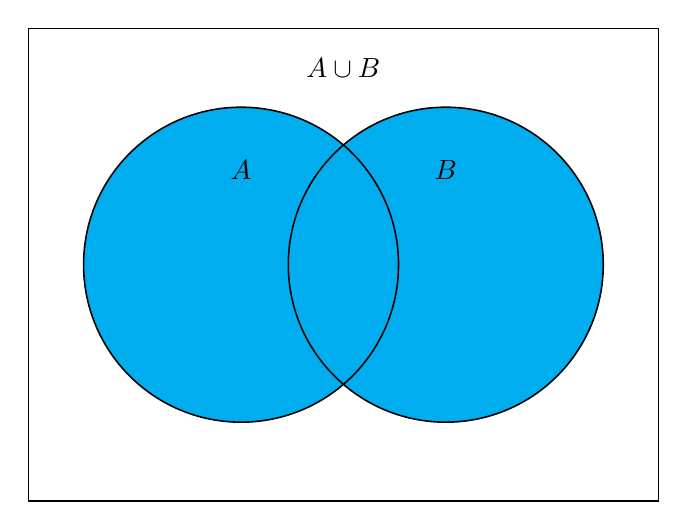
\begin{tikzpicture}[line width=0.2mm]

    % Coordinates for the centers of the circles.
    \coordinate (C1) at (-1.3, 0);
    \coordinate (C2) at ( 1.3, 0);

    % Coordinates for the labels.
    \coordinate (A) at (-1.3, 1.2);
    \coordinate (B) at ( 1.3, 1.2);
    \coordinate (U) at ( 0.0, 2.5);

    % Rectangle indicating the universe set.
    \draw (-4, -3) rectangle (4, 3);

    % Fill in the circle with cyan.
    \draw[fill=cyan, draw=none] (C1) circle (2);
    \draw[fill=cyan, draw=none] (C2) circle (2);

    % Give outlines to the circles.
    \draw (C1) circle (2);
    \draw (C2) circle (2);

    % Labels.
    \node at (A) {$A$};
    \node at (B) {$B$};
    \node at (U) {$A\cup{B}$};
\end{tikzpicture}
                \caption{Venn Diagram for the Union of Two Sets}
                \label{fig:Elem_Alg_Venn_Diagram}
            \end{figure}
            \begin{theorem}
                \label{thm:Elem_Alg_Union_of_Subset}
                If $A$ and $B$ are sets, and $A\subseteq{B}$,
                then $A\cup{B}=B$.
            \end{theorem}
            \begin{proof}
                For if $x\in{A\cup{B}}$, then by definition
                either $x\in{A}$ or $x\in{B}$, or both. But
                if $A\subseteq{B}$, then for all $x\in{A}$, it is
                true that $x\in{B}$. Thus, if $x\in{A}\cup{B}$
                then $x\in{B}$ and therefore
                $A\cup{B}\subseteq{B}$. But if $x\in{B}$, then
                $x\in{A}\cup{B}$ by definition. Therefore
                $B\subseteq{A}\cup{B}$. Thus, from the definition
                of equality, $A\cup{B}=B$.
            \end{proof}
            \begin{theorem}
                \label{thm:Elem_Alg_Intersection_of_Subset}
                If $A$ and $B$ are sets, and $A\subseteq{B}$,
                then $A\cap{B}=A$.
            \end{theorem}
            \begin{proof}
                For if $x\in{A}\cap{B}$, then by
                definition $x\in{A}$ and $x\in{B}$,
                and therefore ${A}\cap{B}\subseteq{A}$.
                But since $A\subseteq{B}$, if
                $x\in{A}$, then $x\in{B}$. That is, if
                $x\in{A}$ then $x\in{A}$ \textbf{and} $x\in{B}$.
                Thus, by definition, $x\in{A}\cap{B}$.
                Therefore $A\subseteq{A}\cap{B}$. Thus, by
                the definition of equality,
                $A\cap{B}=A$.
            \end{proof}
            Theorems \ref{thm:Elem_Alg_Union_of_Subset} and
            \ref{thm:Elem_Alg_Intersection_of_Subset} can best
            be shown using Venn Diagrams. This is shown
            in Fig.~\ref{fig:Elem_Alg_Venn_Diagram_for_Subset}.
            Combining some of these theorem, we obtain the
            following:
            \par
            \vspace{1ex}
            \begin{subequations}
                \begin{minipage}{0.49\textwidth}
                    \begin{equation}
                        A\cap{B}\subseteq{A}\subseteq{A}\cup{B}
                    \end{equation}
                \end{minipage}
                \hfill
                \begin{minipage}{0.49\textwidth}
                    \begin{equation}
                        A\cap{B}\subseteq{B}\subseteq{A}\cup{B}
                    \end{equation}
                \end{minipage}
            \end{subequations}
            \par
            \begin{figure}[H]
                \captionsetup{type=figure}
                \centering
                \begin{subfigure}[b]{0.49\textwidth}
                    \captionsetup{type=figure}
                    \centering
                    %--------------------------------Dependencies----------------------------------%
%   tikz                                                                       %
%-------------------------------Main Document----------------------------------%
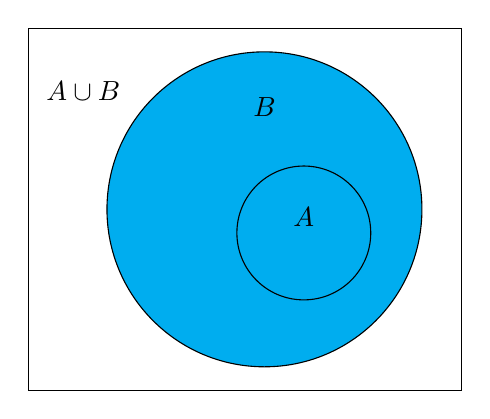
\begin{tikzpicture}
    \draw (-3,-2.3) rectangle (2.5,2.3);
    \draw[fill=cyan] (0,0) circle (2);
    \draw (0.5,-0.3) circle (0.85);
    \node at (0.5,-0.1) {$A$};
    \node at (0,1.3) {$B$};
    \node at (-2.3,1.5) {$A\cup{B}$};
\end{tikzpicture}
                    \subcaption{The Union of Sets $A$ and $B$.}
                    \label{fig:Elem_Alg_Union_of_Subset}
                \end{subfigure}
                \begin{subfigure}[b]{0.49\textwidth}
                    \captionsetup{type=figure}
                    \centering
                    \documentclass[crop,class=article]{standalone}
%----------------------------Preamble-------------------------------%
\usepackage{tikz}                       % Drawing/graphing tools.
%--------------------------Main Document----------------------------%
\begin{document}
    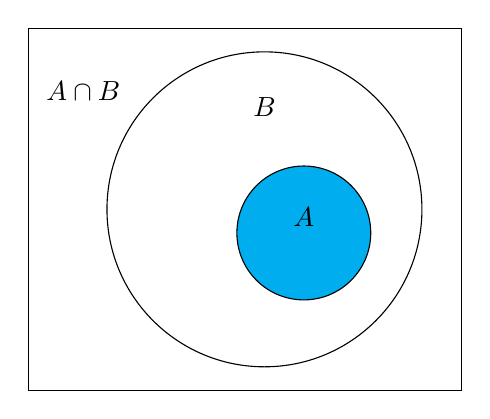
\begin{tikzpicture}
        \draw (-3,-2.3) rectangle (2.5,2.3);
        \draw (0,0) circle (2);
        \draw[fill=cyan] (0.5,-0.3) circle (0.85);
        \node at (0.5,-0.1) {$A$};
        \node at (0,1.3) {$B$};
        \node at (-2.3,1.5) {$A\cap{B}$};
    \end{tikzpicture}
\end{document}
                    \subcaption{The Intersections of Sets
                                $A$ and $B$.}
                    \label{fig:Elem_Alg_Intersection_of_Subset}
                \end{subfigure}
                \caption[More Venn Diagrams]
                        {Venn Diagrams for the
                         Union and Intersection of Two
                         Sets $A$ and $B$ When
                         $A\subseteq{B}$.}
                \label{fig:Elem_Alg_Venn_Diagram_for_Subset}
            \end{figure}
            It is often best to explain mathematics via
            examples. As such, plenty of examples of
            set unions and set intersections are given
            below. The reader should verify some of these
            examples and study the figures given.
            \begin{fexample}{Unions and Intersections}{}
                Below are examples of the union and intersection
                of many different sets.
                \vspace{-2ex}
                \begin{subequations}
                    \begin{align}
                        \{1,2,3,4,5\}\cup\{3,4,5,6,7\}
                        &=\{1,2,3,4,5,6,7\}\\
                        \{3,4,5\}\cup\{1,2,3,4,5\}
                        &=\{1,2,3,4,5\}\\
                        \{0,1,2,3,4\}\cup\{5,6,7,8,9\}
                        &=\{0,1,2,3,4,5,6,7,8,9\}\\
                        \{1,2,3\}\cup\{3,4,5\}&=\{1,2,3,4,5\}\\
                        \{a,b,c\}\cup\{c,d,e\}&=\{a,b,c,d,e\}\\
                        \{\textrm{Boston, Seattle}\}\cup
                        \{\textrm{Seattle}\}
                        &=\{\textrm{Boston, Seattle}\}\\
                        \{\textrm{Bear, Spongebob}\}
                        \cup\{\mathcal{L}\}&=
                        \{\textrm{Bear, Spongebob},
                        \mathcal{L}\}\\
                        \{1,2,3,4,5\}\cap\{3,4,5,6,7\}
                        &=\{3,4,5\}\\
                        \{3,4,5\}\cap\{1,2,3,4,5\}
                        &=\{3,4,5\}\\
                        \{0,1,2,3,4\}\cap\{5,6,7,8,9\}
                        &=\emptyset\\
                        \{1,2,3\}\cap\{3,4,5\}&=\{3\}\\
                        \{a,b,c\}\cap\{c,d,e\}&=\{c\}\\
                        \{\textrm{Boston, Seattle}\}\cap
                        \{\textrm{Seattle}\}
                        &=\{\textrm{Seattle}\}\\
                        \{\textrm{Bear, Spongebob}\}
                        \cap\{\mathcal{L}\}&=\emptyset
                    \end{align}
                \end{subequations}
            \end{fexample}
            The next two topics to discuss are those of
            set difference and symmetric difference. Set
            difference is similar to the concept of subtraction
            that is found in basic arithmetic, with some subtle
            differences. Symmetric difference is defined in terms
            of union, intersection, and set difference and is
            thus the last operation presented.
            \begin{fdefinition*}
                  {Set Difference and Symmetric Difference}{}
                \begin{definition}
                    The set difference of a set $A$ with respect
                    to a set $B$, denoted $A\setminus{B}$,
                    is the set:
                    \begin{equation*}
                        A\setminus{B}=
                        \{x\in{A}:x\notin{B}\}
                    \end{equation*}
                \end{definition}
                \begin{definition}
                    The symmetric difference of two sets $A$ and
                    $B$, denoted $A\ominus{B}$, is the set:
                    \begin{equation*}
                        A\ominus{B}=
                        (A\cup{B})\setminus(A\cap{B})
                    \end{equation*}
                \end{definition}
            \end{fdefinition*}
            The set difference of a set $A$ with respect to a
            set $B$ is the set of all elements in $A$ that are
            not in $B$. In a way, the elements of $B$ are
            \textit{subtracted} from $A$. The analogy is not
            perfect, unfortunately. In arithmetic one
            can subtract a large positive number from a small
            positive number and get a \textrm{negative} number.
            There are, however, no negative sets. If $A$ is a
            subset of $B$, then $A\setminus{B}$ is the empty set.
            \begin{theorem}
                \label{thm:Subset_of_Set_Difference}%
                If $A$ and $B$ are sets, then $A\setminus{B}\subseteq{A}$.
            \end{theorem}
            \begin{proof}
                For if $x\in{A}\setminus{B}$, then
                $x\in{A}$ and $x\notin{B}$. But then
                $x\in{A}$ and therefore, by
                the definition of subsets,
                $A\setminus{B}\subseteq{A}$.
            \end{proof}
            \begin{theorem}
                If $A$ and $B$ are sets and $A\cap{B}=\emptyset$,
                then $A\setminus{B}=A$.
            \end{theorem}
            \begin{proof}
                For if $x\in{A}$, then $x\notin{B}$, since
                $A\cap{B}=\emptyset$. But then, by the definition of set
                difference, $x\in{A}\setminus{B}$. Therefore
                $A\subseteq{A}\setminus{B}$. But by
                Thm.~\ref{thm:Subset_of_Set_Difference},
                $A\setminus{B}\subseteq{A}$. Thus, by the definition of
                equality, $A\setminus{B}=A$.
            \end{proof}
            \begin{theorem}
                If $A$ and $B$ are sets and $A\subseteq{B}$,
                then $A\setminus{B}=\emptyset$.
            \end{theorem}
            \begin{proof}
                For if $A\subseteq{B}$, then for all
                $x\in{A}$ it is true that $x\in{B}$. But then
                there is no element such that
                $x\in{A}$ and $x\notin{B}$, and therefore, by
                the definition of set difference and by the
                definition of the empty set,
                $A\setminus{B}=\emptyset$.
            \end{proof}
            Symmetric difference has a complicated definition
            but an intuitive meaning. It is the set of all
            elements in $A$ or $B$, but not in both.
            Venn Diagrams can be used to visualize set
            differences and symmetric differences, as is shown in
            Fig.~\ref{fig:Elem_Alg_Venn_Diagram_Differences}.
            \begin{figure}[H]
                \captionsetup{type=figure}
                \centering
                \begin{subfigure}[b]{0.49\textwidth}
                    \captionsetup{type=figure}
                    \centering
                    %--------------------------------Dependencies----------------------------------%
%   tikz                                                                       %
%-------------------------------Main Document----------------------------------%
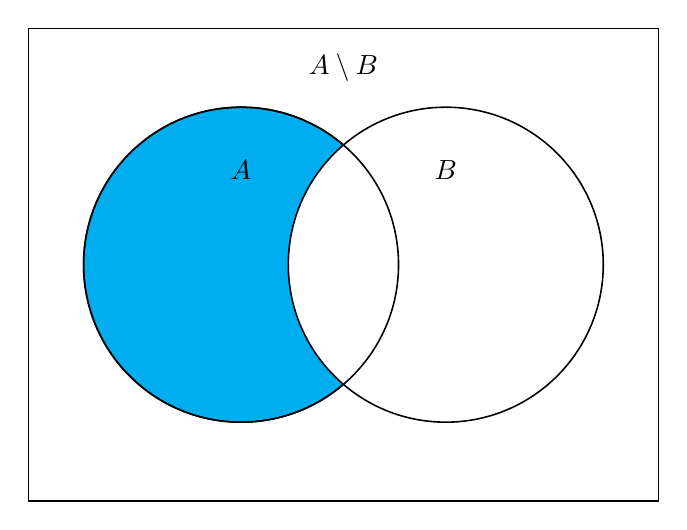
\begin{tikzpicture}[line width=0.2mm]

    % Coordinates for the centers of the circles.
    \coordinate (C1) at (-1.3, 0);
    \coordinate (C2) at ( 1.3, 0);

    % Coordinates for the labels.
    \coordinate (A) at (-1.3, 1.2);
    \coordinate (B) at ( 1.3, 1.2);
    \coordinate (U) at ( 0.0, 2.5);

    % Rectangle indicating the universe set.
    \draw (-4, -3) rectangle (4, 3);

    % Draw the two circles.
    \draw[fill=cyan]              (C1) circle (2);
    \draw[fill=white, draw=black] (C2) circle (2);

    % Add an outline to the left circle.
    \draw (C1) circle (2);

    % Labels.
    \node at (A) {$A$};
    \node at (B) {$B$};
    \node at (U) {$A\setminus{B}$};
\end{tikzpicture}
                    \subcaption{The Set Difference of $A$ and $B$.}
                    \label{fig:Elem_Alg_Set_Difference}
                \end{subfigure}
                \begin{subfigure}[b]{0.49\textwidth}
                    \captionsetup{type=figure}
                    \centering
                    %--------------------------------Dependencies----------------------------------%
%   tikz                                                                       %
%-------------------------------Main Document----------------------------------%
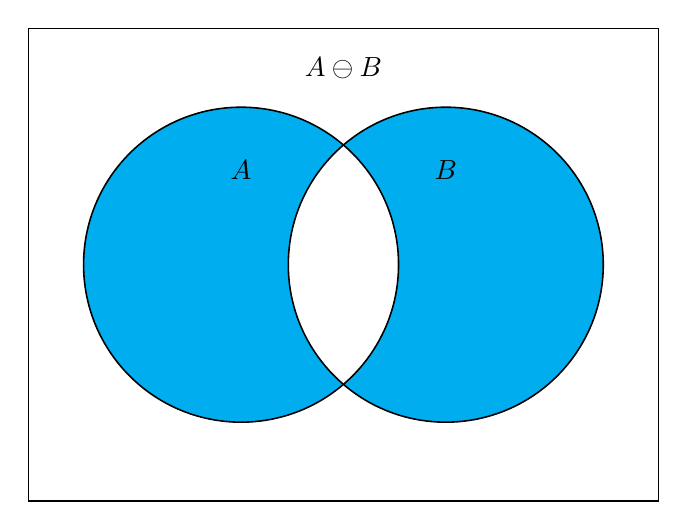
\begin{tikzpicture}[line width=0.2mm]

    % Coordinates for the centers of the circles.
    \coordinate (C1) at (-1.3, 0);
    \coordinate (C2) at ( 1.3, 0);

    % Coordinates for the labels.
    \coordinate (A) at (-1.3, 1.2);
    \coordinate (B) at ( 1.3, 1.2);
    \coordinate (S) at ( 0.0, 2.5);

    % Rectangle indicating the universe set.
    \draw (-4, -3) rectangle (4, 3);

    % Fill in the circle with cyan.
    \draw[fill=cyan, draw=none] (C1) circle (2);
    \draw[fill=cyan, draw=none] (C2) circle (2);

    % Fill in the circle with cyan.
    \draw[fill=white, draw=none] (0, -1.51987) arc(-49.46:49.46:2)
                                               arc(130.54:229.46:2);

    % Give outlines to the circles.
    \draw (C1) circle (2);
    \draw (C2) circle (2);

    % Labels.
    \node at (A) {$A$};
    \node at (B) {$B$};
    \node at (S) {$A\ominus{B}$};
\end{tikzpicture}
                    \subcaption{Symmetric Difference of $A$ and $B$.}
                    \label{fig:Elem_Alg_Symmetric_Difference}
                \end{subfigure}
                \caption[Venn Diagrams for Various Set Operations]
                        {Venn Diagrams for the Set Difference
                         and Symmetric Difference of $A$ and $B$.}
                \label{fig:Elem_Alg_Venn_Diagram_Differences}
            \end{figure}
            \begin{fexample}
                  {Set Difference and Symmetric Difference}{}
                Let's solidify our understanding
                with some examples:
                \begin{align*}
                    \{1,2,3\}\setminus\{1,2\}&=\{3\}\\
                    \{\textrm{Apple, Bob}\}\setminus
                    \{\textrm{Carl, Joe}\}
                    &=\{\textrm{Apple, Bob}\}\\
                    \{1,2,3,4\}\setminus\{1,2,3,4,5,6\}
                    &=\emptyset\\
                    \mathbb{N}_{0}\setminus\mathbb{N}&=\{0\}\\
                    \mathbb{Z}\setminus\mathbb{N}&=
                    \{\hdots,-3,-2,-1,0\}
                \end{align*}
                Recall that $\mathbb{N}_{0}=\{0,1,2,3,\hdots\}$
                and $\mathbb{N}=\{1,2,3,\hdots\}$.
                Taking the difference, we see that that
                only element of $\mathbb{N}_{0}$ that
                is not also contained in $\mathbb{N}$ is 0.
                Therefore
                $\mathbb{N}_{0}\setminus\mathbb{N}=\{0\}$.
                When computing
                $\mathbb{Z}\setminus\mathbb{N}$
                we see that only the positive integers
                are subtracted out, leaving 0 and all of
                the negative integers.
                \begin{align*}
                    \{1,2,3\}\ominus\{1,2,3,4,5,6\}
                    &=\{1,4,5,6\}\\
                    \mathbb{N}_{0}\ominus\mathbb{N}&=\{0\}\\
                    \{\textrm{Apple, Bob}\}\ominus
                    \{\textrm{Carl, Joe}\}
                    &=\{\textrm{Apple, Bob, Carl, Joe}\}\\
                    \{a,b,c\}\ominus\{a,b,c\}&=\emptyset
                \end{align*}
            \end{fexample}
            It is important to note that set difference is
            not a \textit{commutative} operation. That is,
            if $A$ and $B$ are sets, then
            $A\setminus{B}$ and $B\setminus{A}$ may not be equal.
            This is similar to basic arithmetic, where
            $a-b$ and $b-a$ may be different numbers. The other
            operations we have seen are commutative.
            \begin{theorem}
                If $A$ and $B$ are sets, then the following
                equations are true:
                \begin{align}
                    A\cup{B}&=B\cup{A}\\
                    A\cap{B}&=B\cap{A}\\
                    A\ominus{B}&=B\ominus{A}
                \end{align}
            \end{theorem}
            The proof of these three equations comes directly
            from the definitions of union, intersection, and
            symmetric difference. Set difference, on the other
            hand, satisfies a different rule. In arithmetic, if
            $a$ and $b$ are \textit{real numbers}, then
            $a-b=b-a$ if and only if $a=b$. Set difference
            follows the same rule.
            \begin{theorem}
                If $A$ and $B$ are sets, then
                $A\setminus{B}=B\setminus{A}$ if and only if
                $A=B$.
            \end{theorem}
            \begin{proof}
                For if $A=B$, then for all $x\in{A}$
                it is true that $x\in{B}$, and thus
                $A\setminus{B}=\emptyset$.
                Similarly, $B\setminus{A}=\emptyset$. Therefore,
                $A\setminus{B}=B\setminus{A}$. Now, if
                $A\setminus{B}=B\setminus{A}$,
                then for all $x\in{A}\setminus{B}$, it true
                that $x\in{B}\setminus{A}$. But then
                $x\in{A}$ and $x\notin{B}$, and
                $x\in{B}$ and $x\notin{A}$, a contradiction.
                Therefore there is no $x$ such that
                $x\in{A}\setminus{B}$, and thus
                $A\setminus{B}=\emptyset$. But then
                $A\subseteq{B}$. Similarly,
                $B\setminus{A}=\emptyset$, and thus
                $B\subseteq{A}$. Therefore, from the definition
                of equality, $A=B$.
            \end{proof}
            From this we see that
            $A\setminus{B}=B\setminus{A}$ if and only if
            $A\setminus{B}=\emptyset$ and
            $B\setminus{A}=\emptyset$. Similarly, $a-b=b-a$
            if and only if $a-b=0$ and $b-a=0$. While this makes
            it very tempting to associate zero with the empty
            set, and set difference with subtraction, it is
            important to note the differences in these concepts.
            There are a few theorems for dealing with the
            symmetric difference:
            \begin{theorem}
                If $A$ and $B$ are sets and
                $A\cap{B}=\emptyset$, then
                $A\ominus{B}=A\cup{B}$.
            \end{theorem}
            \begin{proof}
                \begin{subequations}
                    From the definition:
                    \begin{equation}
                        A\ominus{B}=
                        (A\cup{B})\setminus(A\cap{B})
                    \end{equation}
                    But $A\cap{B}=\emptyset$, and therefore:
                    \begin{equation}
                        A\ominus{B}=
                        (A\cup{B})\setminus\emptyset
                    \end{equation}
                    But the empty set contains no elements,
                    and therefore
                    $(A\cup{B})\setminus\emptyset=A\cup{B}$. Thus:
                    \begin{equation}
                        A\ominus{B}=A\cup{B}
                    \end{equation}
                \end{subequations}
            \end{proof}
            \begin{theorem}
                If $A$ and $B$ are sets, and if
                $A\subseteq{B}$, then
                $A\ominus{B}=B\setminus{A}$.
            \end{theorem}
            \begin{proof}
                From the definition:
                \begin{equation*}
                    A\ominus{B}=(A\cup{B})\setminus(A\cap{B})
                \end{equation*}
                But from
                Thm.~\ref{thm:Elem_Alg_Union_of_Subset}, if
                $A\subseteq{B}$, then $A\cup{B}=B$. And from
                Thm.~\ref{thm:Elem_Alg_Intersection_of_Subset},
                if $A\subseteq{B}$, then $A\cap{B}=A$. Thus:
                \begin{equation*}
                    (A\cup{B})\setminus(A\cap{B})
                    =B\setminus{A}
                \end{equation*}
            \end{proof}
    \section{Numbers}
        There are many kinds of numbers,
        but certain ones are particularly interesting.
        These sets have a standard notation
        that is agreed upon by most mathematicians.
        \begin{fnotation}{Sets of Numbers}{}
            The Natural numbers.
            \begin{equation*}
                \mathbb{N}=\{1,2,3,4,\hdots\}
            \end{equation*}
            The Whole Numbers.
            \begin{equation*}
                \mathbb{N}_{0}=\{0,1,2,3,4,\hdots\}
            \end{equation*}
            The Integers.
            \begin{equation*}
                \mathbb{Z}=\{\hdots,-2,-1,0,1,2,\hdots\}
            \end{equation*}
            The Rational Numbers.
            \begin{equation*}
                \mathbb{Q}=\{p/q:p,q\in\mathbb{Z},q\ne{0}\}
            \end{equation*}
            The Real Numbers.
            \begin{equation*}
                \mathbb{R}=\{x:x\textrm{ is real.}\}
            \end{equation*}
            The irrational numbers.
            \begin{equation*}
                \mathbb{R}\setminus\mathbb{Q}
                =\{x\in\mathbb{R}:x\notin\mathbb{Q}\}
            \end{equation*}
        \end{fnotation}
        The only serious disagreement that one may find
        is with $\mathbb{N}_{0}$. Computer scientists
        often define $\mathbb{N}$ to include $0$,
        but they're crazy, and some mathematicians write
        $\mathbb{W}=\{0,1,2,3,\hdots\}$
        ($\mathbb{W}$ for \textit{whole} numbers) but they're
        also crazy. While no mathematician would disagree that
        $\mathbb{R}\setminus\mathbb{Q}$ is certainly the set
        of irrational numbers, some (Also crazy) individuals
        choose to write $\mathbb{I}$ to represent this.
        $\mathbb{Z}$, $\mathbb{Q}$, and $\mathbb{R}$ are
        universally accepted. $\mathbb{Z}$ stands for
        \textit{Zahl}, which is German for number.
        $\mathbb{Q}$ stands for \textit{quotient}, since
        rational numbers are quotients of integers. Finally,
        $\mathbb{R}$ simply means \textit{real}.
        From the definitions given, we have the
        following:
        \begin{subequations}
            \begin{equation}
                \mathbb{N}
                \subset\mathbb{N}_{0}
                \subset\mathbb{Z}
                \subset\mathbb{Q}
                \subset\mathbb{R}
            \end{equation}
            \begin{equation}
                \mathbb{R}\setminus\mathbb{Q}
                \subset\mathbb{R}
            \end{equation}
        \end{subequations}
        One might note that, simply by definition, none of the
        rational numbers are irrational and none of the
        irrational numbers are rational.
        $0.111\hdots$ is just a fancy way to write $\frac{1}{9}$.
        Strange beings like $\pi$ are included in the real numbers,
        but cannot be expressed as fractions. It can be shown that
        any rational number has a repeating decimal expansion.
        Therefore a number like:
        \begin{equation}
            C=0.1234567891011121314151617181920\dots
        \end{equation}
        Cannot possibly be rational, for the decimal never repeats.
        For the curious, this number is called
        \textit{Champernowne's Constant}, named after David
        G. Champernowne, who discovered this number in 1933.
        In a similar manner, a number such as:
        \begin{equation}
            q=0.123412341234\cdots
        \end{equation}
        Must be a rational number, for its decimal expansion
        repeats. Using more advanced methods from the study
        of \textit{infinite series}, it can be shown that:
        \begin{equation}
            q=\frac{1234}{9999}
        \end{equation}
        The real numbers are often visualized as lying on a
        line, and indeed are often called the \textit{real line}.
        This visual gives us an intuitive way to order the numbers,
        by saying that $x$ is \textit{less than} $y$ if $x$ is
        to the left of $y$ on the number line. Similarly, we say
        that $x$ is \textit{greater than} $y$ if $x$ is to the
        right of $y$ on the number line.
        \begin{properties}[Order Property of Real Numbers]
            For two real numbers $a,b\in \mathbb{R}$:
            \begin{enumerate}
                \item $a<b$ if $a$ is to the left of $b$ on the number line.
                \item $a>b$ if $a$ is to the right of $b$ on the number line.
            \end{enumerate}
        \end{properties}
        \begin{definition}
        A variable is a symbol used to represent an unknown quantity.
        \end{definition}
        \begin{example}
        $x$ and $y$ are commonly used to represent real numbers. $n$ and $m$ are commonly used to represent integers. $z$ is often used to represent complex numbers, but we won't get into that until later.
        \end{example}
        \begin{example}
        Let's use a variable to represent the sentence "To hit a baseball out of the park, the ball must travel more than 315 feet." Let $d$ be the distance the ball must travel to be a home run. Then $d>315$
        \end{example}
        \begin{notation}
        If we wish to say $a$ is less than or equal to $b$, we write $a\leq b$. This means that either $a<b$ or $a=b$. Similarly, if we wish to write that $a$ is greater than or equal to $b$, we write $a\geq b$. This means that either $a>b$ or $a=b$.
        \end{notation}
        The absolute value of a real number is the distance from that number to the origin (The number $0$).
        \begin{definition}
            The absolute value of a real number
            $x\in \mathbb{R}$ is:
            \begin{equation}
                |x|=
                \begin{cases}
                    x,&x\geq{0}\\
                    \minus{x},&x<0
                \end{cases}
            \end{equation}
        \end{definition}
        \begin{theorem}
        If $a$ and $b$ are real numbers,
        then the following are true:
            \begin{enumerate}
                \begin{multicols}{2}
                \item $|a+b|=|-a-b|$
                \item $|a-b|=|b-a|$
                \item $|\minus{a}|=|a|$
                \item $|a\cdot{b}|=|a|\cdot|b|$
                \end{multicols}
            \end{enumerate}
        \end{theorem}
        \begin{lexample}{}{}
            Let's compute the absolute value of various numbers.
            If $x$ is a real number, and $x>0$, then
            $|x|=x$. For example:
            \par
            \begin{subequations}
                \begin{align}
                    |1|&=1\\
                    |\tfrac{3}{4}|&=\tfrac{3}{4}\\
                    |\pi|&=\pi\\
                    |\sqrt{2}|&=\sqrt{2}
                \end{align}
            \end{subequations}
            If $x<0$, then $|x|=\minus{x}$. This may be confusing,
            so instead of $x<0$ write $x=\minus{y}$, where $y$
            is positive. From this we get $|x|=y$. For example:
            \begin{subequations}
                \begin{align}
                    |\minus1|&=1\\
                    |\minus\tfrac{3}{4}|&=\tfrac{3}{4}\\
                    |\minus\pi|&=\pi\\
                    |\minus\sqrt{2}|&=\sqrt{2}
                \end{align}
            \end{subequations}
            For products $z=x\cdot{y}$, we can compute $|z|$ by
            computing the $|x|$ and $|y|$ separately, and then
            multiplying the final results. That is, $|z|=|x|\cdot|y|$.
            For example:
            \begin{subequations}
                \begin{align}
                    |(\minus{3})\cdot4|&=12\\
                    |(\minus{3})\cdot(\minus{4})|&=12
                \end{align}
                The absolute value of a real number is always positive.
                Intuitively, one can think of this as the
                \textit{distance} from a real number $x$ to zero. Zero
                is also called the \textit{origin} of the real number line,
                so $|x|$ is the distance from $x$ to the origin.
            \end{subequations}
        \end{lexample}
        \begin{definition}
            The exponentiation of a real number $a\in \mathbb{R}$ by a
            natural number $n\in \mathbb{N}$ is the number:
            \begin{equation}
                a^{n}=\underset{n\textrm{ times}}{\underbrace{a\cdots{a}}}
            \end{equation}
        \end{definition}
        \begin{example}[Examples of Exponentiation]
        \
        \begin{enumerate}
        \begin{multicols}{2}
        \item $10^2 = 10\cdot 10 = 100$.
        \item $10^4 = 10\cdot 10 \cdot 10 \cdot 10 = 10000$
        \item $10^1 = 10$
        \item $2^3 = 2\cdot 2 \cdot 2 = 8$
        \item $\pi^2 = \pi\cdot \pi = 9.869\hdots$
        \item $(\sqrt{2})^2 = \sqrt{2}\cdot \sqrt{2} = 2$.
        \end{multicols}
        \end{enumerate}
        \end{example}
        The fact that $(\sqrt{2})^2=2$ is really the definition of the number $\sqrt{2}$. We'll see this in a bit.
        \begin{theorem}
         The following are true:
            \begin{enumerate}
                \begin{multicols}{2}
                    \item If $n\in \mathbb{N}$, then $0^n = 0$.
                    \item $(-1)^2 = 1$
                    \item $(-x)^2 = x^2$
                    \item $(-1)^3 = -1$
                    \item $(-x)^3=-x^3$
                    \item If $n$ is even, then $(-1)^n = 1$
                    \item if $n$ is even, then $(-x)^n = x^n$
                    \item If $n$ is odd, then $(-1)^n = -1$
                    \item If $n$ is odd, then $(-x)^n = -x^n$. 
                \end{multicols}
            \end{enumerate}
        \end{theorem}
        \begin{theorem}
        If $y$ is a positive real number, then there is a unique positive real number $x$ such that $y=x^2$.
        \end{theorem}
        The theorem says there is a unique $positive$ real number. There are actually two real numbers satisfying this property. For if $y=x^2$, then $y=(-x)^2$, and thus $x$ and $-x$ are solutions. One of these will be negative, though.
        \begin{definition}
        The principal square root of a positive real number $x$, denoted $\sqrt{x}$, is the unique positive real number such that $(\sqrt{x})^2 = x$. The symbol $\sqrt{\ \ }$ is called a radical, and $x$ is called the radicand.
        \end{definition}
        \begin{example}[Examples of Square Roots]
        \
        \begin{enumerate}
        \begin{multicols}{4}
        \item $\sqrt{1} = 1$
        \item $\sqrt{4} = 2$
        \item $\sqrt{9} = 3$
        \item $\sqrt{16} = 4$
        \item $\sqrt{25} = 5$
        \item $\sqrt{36} = 6$
        \item $\sqrt{49} = 7$
        \item $\sqrt{64} = 8$
        \end{multicols}
        \end{enumerate}
        \end{example}
        \begin{theorem}
        If $y\in \mathbb{R}$ is a real number, then there is a unique real number $x$ such that $y=x^3$.
        \end{theorem}
        \begin{definition}
        The cube root of a real number $x$, denoted $\sqrt[3]{x}$, is the unique real number such that $(\sqrt[3]{x})^3 = x$.
        \end{definition}
        \begin{example}[Examples of Cube Roots]
        \
        \begin{enumerate}
        \begin{multicols}{4}
        \item $\sqrt[3]{-1} = -1$
        \item $\sqrt[3]{8} = 2$
        \item $\sqrt[3]{-8} = -2$
        \item $\sqrt[3]{27} = 3$
        \item $\sqrt[3]{125} = 5$
        \item $\sqrt[3]{-125} = -5$
        \item $\sqrt[3]{-64} = -4$
        \item $\sqrt[3]{1000} = 10$
        \end{multicols}
        \end{enumerate}
        \end{example}
        The cube root theorem is more relaxed than the square root theorem. The square root theorem requires that $y$ is positive. Negative real numbers do not have square roots. However, all real number have cube roots.
        Note that for any positive real number $a$, $\big(\sqrt{a}\big)^2 = a$, and for any real number $b$, $(\sqrt[3]{b})^3 = b$.
        \begin{theorem}
        If $r\in \mathbb{R}$ is positive and $n\in \mathbb{N}$, then there is a unique positive real number $\sqrt[n]{r}$, such that $(\sqrt[n]{r})^n = r$.
        \end{theorem}
        \begin{definition}
        The principal $n^{th}$ root of a positive $r\in \mathbb{R}$ is the unique positive real number such that $(\sqrt[n]{r})^n = r$.
        \end{definition}
        \begin{example}[Examples of $n^{th}$ Roots]
        \
        \begin{enumerate}
        \begin{multicols}{4}
        \item $\sqrt{4} = 2$
        \item $\sqrt[3]{27} = 3$
        \item $\sqrt[4]{16} = 2$
        \item $\sqrt[3]{125} = 5$
        \item $\sqrt[3]{8} = 2$
        \item $\sqrt[4]{81} = 3$
        \item $\sqrt[5]{32} = 2$
        \item $\sqrt[6]{729} = 3$
        \end{multicols}
        \end{enumerate}
        \end{example}
        \begin{properties}[The Order of Operations]
        When performing arithmetic to simplify expressions, use the following order:
        \begin{enumerate}
        \item Perform operations inside parenthesis, brackets, braces, etc., first.
        \item Next, perform exponentiation.
        \item Then perform multiplication and division from left to right in the order they appear in the expression.
        \item Finally perform addition and subtraction from left to right in the order they appear in the expression.
        \end{enumerate}
        \end{properties}
        For some reason, the internet was once obsessed with the expression $48\div 2(9+3)$. Depending on what
        you do, you either got $288$ or $2$. According to the order of operations, the $correct$ answer
        is $288$. However the $real$ correct answer is: \textbf{If you write ambiguous expressions like this
        instead of using parantheses, then you are a bad person}. Parenthesis rid of ambiguity.
        $48\div\big(2(9+3)\big) = 2$, unambiguously. $\big(48\div 2\big)(9+3) = 288$, again unambiguously.
        Furthermore, stop using the $\div$ symbol. It's archaic and ambiguous. Writing $\frac{48}{2(9+3)}$
        or $\frac{48}{2}(9+3)$ leaves no ambiguity.
        \subsubsection{Solved Problems}
        \begin{enumerate}
        \begin{multicols}{4}
        \item $|-2.75| = 2.75$
        \item $|-7.24| = 7.24$
        \item $-|-4| = -4$
        \item $-|-6| = -6$
        \item $|3-(-6)| = 9$
        \item $|-4-7| = 11$
        \item $|-7.5-2.5| = 10$
        \item $|13.4 - (-2.6)| = 16$
        \item $|5-2| = 3$
        \item $|-1-2| = 3$
        \item $7^2 = 49$
        \item $(-7)^2 = 49$
        \item $-7^2 = -49$
        \item $-(-7)^2 = -49$.
        \item $3^3 = 27$
        \item $(-3)^3 = -27$
        \item $-(-3)^3 = 27$
        \item $(-1)^2 = 1$
        \item $(-1)^3 = -1$
        \item $(-1)^4 = 1$
        \item $(-1)^5 = -1$
        \item $-24 - (-31) = 7$
        \item $\frac{-\frac{3}{4}}{\frac{7}{8}} = -\frac{6}{7}$
        \item $\frac{-20}{\frac{1}{2}} = -40$.
        \end{multicols}
        \end{enumerate}
        \subsubsection{Algebraic Expressions and the Properties of Real Numbers}
        \begin{definition}
        An algebraic term is a collection of factors such as numbers, variables, or expressions within parentheses.
        \end{definition}
        \begin{example}[Examples of Algebraic Terms]
        \
        \begin{enumerate}
        \begin{multicols}{6}
        \item $3$
        \item $-x$
        \item $5xy$
        \item $-3n^3$
        \item $4y$
        \item $2(x+3)$.
        \end{multicols}
        \end{enumerate}
        \end{example}
        \begin{definition}
        The numerical value in a term is called its coefficient.
        \end{definition}
        \begin{example}[Examples of Coefficients]
        \
        \begin{enumerate}
        \begin{multicols}{3}
        \item $4$ is the coefficient of $4xy$
        \item $3$ is the coefficient of $3z^2$
        \item $1$ is the coefficient of $xyz$
        \item $\frac{1}{\pi}$ is the coefficient of $\frac{1}{p}x^3$.
        \item $1$ is the coefficient of $x$
        \item $10$ is the coefficient of $10t^2$
        \end{multicols}
        \end{enumerate}
        \end{example}
        \begin{definition}
        A constant is an algebraic term with only a numerical factor in it.
        \end{definition}
        \begin{definition}
        A variable term is an algebraic term that contains a variable.
        \end{definition}
        \begin{example}[Examples of Variable Terms]
        \
        \begin{enumerate}
        \begin{multicols}{4}
        \item $x^2$
        \item $2xyz^2$
        \item $5t^4$
        \item $3x(y+1)$
        \item $t(x+y)(x-y)$
        \item $3t^2y$
        \item $x^4y^3z^2w$
        \item $2\pi r$
        \end{multicols}
        \end{enumerate}
        \end{example}
        \begin{definition}
        An algebraic expression is a single term or the sum of finitely many terms.
        \end{definition}
        \begin{example}
        Let's translate the following sentences into mathematical expressions:
        \begin{enumerate}
        \begin{multicols}{2}
        \item Twice a number, increased by $5$: $2n+5$
        \item Six less than three times a number: $3n-6$
        \end{multicols}
        \end{enumerate}
        \end{example}
        \begin{properties}[Evaluating a Mathematical Expression]
        To evaluate an expression, do the following:
        \begin{enumerate}
        \begin{multicols}{2}
        \item Substitute the given values for each variable.
        \item Simplify.
        \end{multicols}
        \end{enumerate}
        \end{properties}
        \begin{example}
        Solve $x^3-2x^2+5$ for $x=-3$: $(-3)^3+2(-3)^2+5 = -27-18+5 = -40$.
        \end{example}
        \begin{properties}[The Commutative Properties]
        If $a$ and $b$ are real numbers, then the following is true:
        \begin{enumerate}
        \item $a+b = b+a$ \hfill [The Commutative Property of Addition]
        \item $a\cdot b = b\cdot a$ \hfill [The Commutative Property of Multiplication]
        \end{enumerate}
        \end{properties}
        \begin{example}[Examples of the Commutative Properties]
        \
        \begin{enumerate}
        \begin{multicols}{3}
        \item $2+3 = 5,\ 3+2 = 5$
        \item $2+(-8) = -6,\ (-8)+2 = - 6$
        \item $5\cdot 6 = 30,\ 6\cdot 5 = 30$
        \end{multicols}
        \end{enumerate}
        \end{example}
        \begin{properties}[The Associative Properties]
        If $a,b,c\in \mathbb{R}$, then the following is true:
        \begin{enumerate}
        \item $a+(b+c) = (a+b)+c$ \hfill [The Associative Property of Addition]
        \item $a\cdot(b\cdot c) = (a\cdot b)\cdot c$ \hfill [The Associative Property of Multiplication]
        \end{enumerate}
        \end{properties}
        \begin{example}[Examples of the Associative Properties]
        \
        \begin{enumerate}
        \begin{multicols}{2}
        \item $1+(2+3) = 1+5 = 6,\ (1+2)+3 = 3+3 = 6$
        \item $5+(2+8) = 5+10 = 15,\ (5+2)+8 = 7+8 = 15$
        \item $2\cdot(3\cdot 4) = 2\cdot 12 = 24,\ (2\cdot 3)\cdot 4 = 6\cdot 4 = 24$
        \item $\frac{1}{2}\cdot(2\cdot 3) = \frac{1}{2}\cdot 6 = 3,\ (\frac{1}{2}\cdot 2)\cdot 3 = 1\cdot 3 = 3$.
        \end{multicols}
        \end{enumerate}
        \end{example}
        \begin{properties}[The Distributive Property of Multiplication over Addition]
        If $a,b,c\in \mathbb{R}$, then the following is true:
        \begin{enumerate}
        \item $a\cdot(b+c) = (a\cdot b) + (a\cdot c)$\hfill [The Distributive Property of Multiplication over Addition]
        \end{enumerate}
        \end{properties}
        \begin{example}[Examples of the Distributive Property]
        \
        \begin{enumerate}
        \item $2\cdot(1+1) = 2\cdot 2 = 4,\ 2\cdot(1+1) = (2\cdot 1)+(2\cdot 1) = 2+2 = 4$
        \item $2\cdot(2+3) = 2\cdot 5 = 10,\ 2\cdot(2+3) = (2\cdot 2)+(2\cdot 3) = 4+6 = 10$
        \end{enumerate}
        \end{example}
        \begin{definition}
        Like terms are two algebraic terms that have the same variable factors.
        \end{definition}
        \begin{example}
        In $xy+x+2xy$, $xy$ and $2x$ are like terms so we can combine them to get $3xy+x$.
        \end{example}
        When trying to simplify an expression, we use the distributive property, the associative properties, and the commutative properties to combine like terms to get and form simplified expressions.
        \begin{enumerate}
        \begin{multicols}{2}
        \item Seven fewer then a number: $n-7$
        \item $x$ decreased by $6$: $x-6$
        \item The number of a number and four: $n+4$
        \item A number increased by $9$: $n+9$
        \item The difference between a number and five is squared: $(n-5)^2$
        \item The sum of a number and two is cubed: $(n+2)^3$
        \item Thirteen less than twice a number: $2n-13$
        \item Five less than double a number: $2n-13$
        \end{multicols}
        \item[] Let $x=2$ and $y=-3$. Evaluate:
        \begin{multicols}{4}
        \item $4x-2y: 14$
        \item $5x-3y: 19$
        \item $-2x^2+3y^2: 19$
        \item $-5x^2+4y^2: 16$
        \item $2y^2+5y-3: 0$
        \item $3x^2+2x-5: 11$
        \item $(2x-2y)^2:144$
        \item $(2x-3y)^2: 169$
        \end{multicols}
        \end{enumerate}
        \subsubsection{Exponents, Scientific Notation, and a Review of Polynomials}
        \begin{notation}
        If $a\in \mathbb{R}$, $a\ne 0$, and $n\in \mathbb{Z}$, $n<0$, then $a^n = \frac{1}{a^{|n|}}$.
        \end{notation}
        \begin{example}[Examples of Negative Exponents]
        \
        \begin{enumerate}
        \begin{multicols}{4}
        \item $2^{-1} = \frac{1}{2}$
        \item $2^{-3} = \frac{1}{2^3} = \frac{1}{8}$
        \item $10^{-1} =\frac{1}{10}$
        \item $10^{-3} = \frac{1}{10^3} = \frac{1}{1000}$
        \item $4^{-2} = \frac{1}{4^2} = \frac{1}{16}$
        \item $\pi^{-1} = \frac{1}{\pi}$
        \item $\pi^{-2} = \frac{1}{\pi^2}$
        \item $\big(\frac{1}{2}\big)^{-1} = 2$
        \item $\big(\frac{3}{2}\big)^{-1} = \frac{2}{3}$
        \item $\big(\frac{1}{10}\big)^{-2} = 10^2 = 100$
        \item $\big(\frac{1}{2}\big)^{-3} = 2^3 = 8$
        \item $\big(\frac{3}{2}\big)^{-4} = \big(\frac{2}{3}\big)^4 = \frac{16}{81}$
        \end{multicols}
        \end{enumerate}
        \end{example}
        \begin{notation}
        If $a \in \mathbb{R}$, $a>0$, and $p,q \in \mathbb{Z}$, then $a^{\frac{p}{q}}$ is the unique positive number such that $\big(a^{\frac{p}{q}}\big)^q = a^p$.
        \end{notation}
        \begin{example}[Examples of Fractional Exponents]
        \
        \begin{enumerate}
        \begin{multicols}{4}
        \item $2^{\frac{1}{2}} = \sqrt{2}$
        \item $2^{\frac{1}{3}} = \sqrt[3]{2}$
        \item $10^{\frac{1}{n}} = \sqrt[n]{10}$
        \item $2^{\frac{3}{2}} = \sqrt{2^3} = \sqrt{8}$
        \item $10^{\frac{4}{3}} = \sqrt[3]{10^4} = \sqrt[3]{10000}$
        \item $3^{\frac{4}{5}} = \sqrt[5]{3^4} = \sqrt[5]{81}$
        \item $2^{\frac{5}{6}} = \sqrt[6]{2^5} = \sqrt[6]{32}$
        \item $6^{\frac{5}{5}} = \sqrt[5]{6^5} = 6$. 
        \end{multicols}
        \end{enumerate}
        \end{example}
        Thus, we have defined exponentiation for negative integers and fractions as well.
        \begin{properties}[The Properties of Exponents]
        If $a,b\in \mathbb{R}$ and $n,m,p\in \mathbb{N}$, then the following are true:
        \begin{enumerate}
        \item $\big(a^n\big)^m = a^{n\cdot m}$ \hfill [Power Property]
        \item $a^n \cdot a^m = a^{n+m}$ \hfill [Product Property]
        \item $\big(a^m\cdot b^n\big)^p = a^{m \cdot p} \cdot b^{n\cdot p}$ \hfill [Product to a Power Property]
        \item If $b\ne 0$, $\big(\frac{a^n}{b^n}\big)^p = \frac{a^{n\cdot p}}{b^{n\cdot p}}$ \hfill [Quotient to a Power Property]
        \item If $a\ne 0$, $\frac{a^n}{a^m} = a^{n-m}$ \hfill [Quotient Property]
        \item If $a\ne 0$, $a^0 = 1$\hfill [The Zero Property]
        \end{enumerate}
        \end{properties}
        WARNING: Some notation from calculus ahead. We leave $0^0$ undefined. In various scenarios in calculus, we use the convention that $0^0 = 1$, but this is no more than a convention. An example is in infinite series. Say we want to add $1+x+x^2+x^3+x^4+\hdots$. We use the notation $\sum_{n=0}^{\infty} x^n=x^0+x^1+x^2+x^3+\hdots$ to represent this. We plug in a value for $x$ and get a number. For every value of $x$ other than $x=0$, we have $x^0 = 1$ and so we get back the original sum. It would be really annoying to continuously talk about the special case when $x=0$, and so we adopt the convention that $0^0 =1$ as well. This is just a convention for this area of mathematics, and $0^0$ is, in general, left undefined.
        \begin{definition}
        The scientific notation of a real number $x$ is $x = r\times 10^n$, where $0\leq |r| < 10$, and $n\in \mathbb{Z}$.
        \end{definition}
        Every real number has a scientific representation.
        \begin{example}[Examples of Scientific Notation]
        \
        \begin{enumerate}
        \begin{multicols}{3}
        \item $101 = 1.01\times 10^2$
        \item $10,000 = 1\times 10^4$
        \item $314.15926\hdots = \pi \times 10^2$
        \item $-123.456 = -1.23456\times 10^2$
        \item $-0.031415926\hdots = -\pi \times 10^{-2}$
        \item $0.00001 = 1\times 10^{-5}$
        \end{multicols}
        \item $0.\underset{33\ times}{\underbrace{0\hdots 0}662607004} = 6.62607004\times 10^{-34} = h$ (Physicist's like this number)
        \end{enumerate}
        \end{example}
        \begin{definition}
        A monomial is a term with only whole number variable exponents and no variables in the denominator.
        \end{definition}
        \begin{example}[Examples of Monomials]
        \
        \begin{enumerate}
        \begin{multicols}{4}
        \item $4x^2$
        \item $3xyz$
        \item $3y^2z$
        \item $3z^2$
        \end{multicols}
        \end{enumerate}
        \end{example}
        \begin{definition}
        A polynomial is a sum of monomials.
        \end{definition}
        \begin{example}[Examples of Polynomials]
        \
        \begin{enumerate}
        \begin{multicols}{4}
        \item $x^2+x+1$
        \item $3xy+6z^2+w$
        \item $x^2+2xy+y^2$
        \item $1+xyz+x^2y^2z^2$
        \end{multicols}
        \end{enumerate}
        \end{example}
        \begin{definition}
        The degree of a polynomial in one variable is the largest exponent of any of the terms.
        \end{definition}
        \begin{definition}
        The degree of a polynomial in many variables is the largest sum of exponents of any of the terms.
        \end{definition}
        \begin{definition}
        A binomial is a polynomial with two monomial terms.
        \end{definition}
        
        \begin{definition}
        A trinomial is a polynomial with three monomial terms.
        \end{definition}
        
        \begin{example}
        \
        \begin{enumerate}
        \begin{multicols}{2}
        \item $5x^2y-2xy$ is a binomial of degree $3$.
        \item $3x^2 - 1$ is a binomial of degree $2$.
        \item $z^3-3z^2+9z-27$ is a polynomial of degree $3$.
        \item $x+5$ is a binomial of degree $1$.
        \item $2x^2+x+3$ is a trinomial of degree $2$.
        \item $xyz+1$ is a binomial of degree $3$
        \item $x^2yz +x+1$ is a trinomial of degree $4$
        \item $x^2y^2z + 1$ is a binomial of degree $5$
        \item $x^2y^2z^2 + 2$ is a binomial of degree $6$
        \item $x^{10} y^{26} z^3 + 2x^2+1$ is a trinomial of degree $39$
        \end{multicols}
        \end{enumerate}
        \end{example}
        To add polynomials, we combine like terms and simplify using the commutative and associative properties.
        \begin{example}[Adding Polynomials]
        \
        \begin{enumerate}
        \item $(3x^2y+x+y)+(2x^2y-y) = 5x^2y+x$
        \item $(1+x+x^2)+(x+x^2+x^3) = 1+2x+2x^2+x^3$
        \item $(1+x)+(x+x^2) = 1+2x+x^2$
        \item $(xyz+xy+x+z) + (y+xz+yz-xyz) = xy+xz+yz+x+y+z$
        \end{enumerate}
        \end{example}
        To multiply two polynomials, we use the distributive property and then combine like terms.
        \begin{example}[Multiplying Polynomials]
        \
        \begin{enumerate}
        \begin{multicols}{2}
        \item $xy(x+z) = x^2y+xyz$
        \item $x(y+z) = xy+xz$
        \item $(x+1)(y^2+z) = xy^2+xz+y^2+z$
        \item $(x+y)(x-y) = x^2-y^2$.
        \end{multicols}
        \end{enumerate}
        \end{example}
        \begin{theorem}
        If $A$ and $B$ are real numbers, the following is true:
        \begin{enumerate}
        \item $(A+B)(A-B) = A^2-B^2$ \hfill [Binomial Conjugates]
        \item $(A+B)^2 = A^2 + 2AB + B^2$ \hfill [Square of a Sum]
        \item $(A-B)^2 = A^2-2AB + B^2$ \hfill [Square of a Difference]
        \end{enumerate}
        \end{theorem}
        \begin{enumerate}
        \begin{multicols}{3}
        \item $n^2\cdot 21n^5= 21n^7$
        \item $5x^2 \cdot 7x^2= 35 x^4$
        \item $(-6p^2q)(2p^3q^3)= -12p^5q^4$
        \item $(a^2)^4\cdot (a^2)^3\cdot b^2\cdot b^5= a^{14}b^7$
        \item $(6pq^2)^3= 216p^3q^6$
        \item $\frac{-6 w^5}{-2 w^2}= 3w^3$
        \item $\frac{8 z^7}{16 z^5}= \frac{1}{2}z^2$
        \item $\frac{-12 a^3b^5}{4a^2b^4}= -3ab$
        \item $\big(\frac{2}{3}\big)^{-3}= \frac{27}{8}$
        \item $\frac{5m^3n^5}{10mn^2}= \frac{1}{2}m^2n^3$
        \item $\frac{3}{m^{-2}}= 3m^2$
        \item $\big(\frac{2p^4}{q^3}\big)^2= 4\frac{p^8}{q^6}$
        \item $\big(\frac{-5 v^4}{7w^3}\big)^2= \frac{25 v^8}{49 w^6}$
        \item $\frac{9p^6 q^4}{-12p^4q^6}= -\frac{3}{4} \frac{p^2}{q^2}$
        \item $\frac{5m^2 n^2}{10 m^2 n}= \frac{1}{2} n$
        \item $\frac{5k^3}{20 k^{-2}}= \frac{1}{4} k^5$
        \item $\frac{7x^3}{x} = 7x^2$
        \item $\frac{x^2y^3 z^4}{xyz} = xy^2z^3$
        \end{multicols}
        \item $(x^3+2x^2+x+1)+(3x^3-4x) = 4x^3+2x^2-3x+1$
        \item $(xy+1)+(3x^2-2xy+4) = -xy+3x^2+5$
        \begin{multicols}{2}
        \item $2x(x^2+y^2) = 2x^3+2xy^2$
        \item $(1+x)(1-x) = 1+x^2$
        \item $(1+x+x^2)(1-x) = 1 - x^3$
        \item $(1+x+x^2+x^3)(1-x) = 1 - x^4$
        \item $(2x^2+3y)(x+y) = 2x^3+2x^2y+3xy+3y^2$
        \item $xy(x+y)^2 = x^3y+2x^2y^2+xy^3$
        \end{multicols}
        \end{enumerate}
        \subsubsection{Factoring Polynomials}
        \begin{definition}
        To factor an expression is to rewrite the expression as an equivalent product.
        \end{definition}
        The distributive property of multiplication over addition is an example of factoring.
        \begin{example}
        Let's factor $x^2+2xy+y^2$. Using the distributive property we obtain $x^2+2xy+y^2=x^2+xy+xy+y^2 = x(x+y)+y(x+y) = (x+y)(x+y) = (x+y)^2$.
        \end{example}
        \begin{example}
        Let's factor $12x^2+18xy-30y$. Using the distributive property, $12x^2+12xy-30y = 6(2x^2+3xy-5y)$.
        \end{example}
        \begin{example}
        $x^5+x^2 = x^2(x^3+1)$.
        \end{example}
        \begin{example}
        Let's factor $3t^3+15t^2-6t-30$. Using the distributive property, we have $3\big(t^3+5t^2-2t-10\big) = 3\big(t^2(2t+5)-2(t+5)\big) = 3\big((t^2-2)(t+5)\big) = 3(t^2-2)(t+5)$.
        \end{example}
        \begin{example}
        $(x+3)x^2+5(x+3) = (x+3)(x^2+5)$.
        \end{example}
        \begin{definition}
        A quadratic polynomial is one of the form $ax^2+bx+c$, where $a,b,c\in \mathbb{R}$.
        \end{definition}
        There is a special case of quadratic polynomials where $a=1$. That is, quadratics of the form $x^2+bx+c$ for real numbers $b,c\in \mathbb{R}$. 
        \begin{theorem}
        If $x^2+bx+c$ is a quadratic, where $b,c\in \mathbb{R}$, and if $\alpha,\beta \in \mathbb{R}$ are real numbers such that $\alpha \cdot \beta = c$ and $\alpha+\beta = b$, then $x^2+bx+c = (x+\alpha)(x+\beta)$.
        \end{theorem}
        \begin{proof}
        For $(x+\alpha)(x+\beta) = x^2+\alpha x + \beta x + \alpha\cdot \beta = x^2+x(\alpha + \beta) + \alpha \cdot \beta=x^2+bx+c$.
        \end{proof}
        \begin{example}
        $x^2-11x+24 = (x-3)(x-8)$.
        \end{example}
        \begin{example}
        $x^2-3x-10 = (x-5)(x+2)$
        \end{example}
        \begin{definition}
        A prime polynomial is a polynomial that cannot be factored further.
        \end{definition}
        \begin{example}
        $x^2+9x+15$ is a prime polynomial. We need $\alpha\cdot \beta = 15$ and $\alpha+\beta = 9$. Factoring $15$ into prime numbers, we get $15 = 5\cdot 3$ or $15 = 15\cdot 1$. In either case, $5+3=8\ne 9$ and $15+1 = 16 \ne 9$. So $x^2+9x+15$ cannot be factored further using integer coefficients.
        \end{example}
        For the general case of $a\ne 0$, we let $d = \frac{b}{a}$ and $e = \frac{c}{a}$. Then we find $\alpha$ and $\beta$ such that $(x+\alpha)(x+\beta) = x^2+dx+e$. Multiplying both sides by $a$ gives us $a(x+\alpha)(x+\beta) = ax^2+adx+ae = ax^2+bx+c$. So, $(ax+a\cdot \alpha)(x+\beta) = ax^2+bx+c$. So the general case reduces to the specific case of $a=1$.
        We've seen the following identities before, and they can be used to simplify expressions:
        \begin{enumerate}
        \item $A^2-B^2 = (A+B)(A-B)$ \hfill [Difference of Squares]
        \item $A^2+2AB+B^2 = (A+B)^2$ \hfill [Square of a Sum]
        \item $A^2-2AB+B^2 = (A-B)^2$ \hfill [Square of a Difference]
        \end{enumerate}
        \begin{example}[Examples of Factoring]
        \
        \begin{enumerate}
        \begin{multicols}{2}
        \item $4x^2-81 = (2x+9)(2x-9)$
        \item $x^2+49$ is prime.
        \item $x^2 - 16 = (x+4)(x-4)$.
        \item $x^2-9 = (x+3)(x-3)$
        \item $x^4 - 81 = (x^2+9)(x^2-9) = (x^2+9)(x+3)(x-3)$.
        \item $4x^2+8xy+4y^2 = (2x)^2+2(2x)(2y)+(2y)^2 = (2x+2y)^2$
        \end{multicols}
        \end{enumerate}
        \end{example}
        There are two identities that help us factor cubes very easily.
        \begin{enumerate}
        \item $x^3+y^3 = (x+y)(x^2-xy+y^2)$ \hfill [Sum of Cubes]
        \item $x^3-y^3 = (x-y)(x^2+xy+y^2)$ \hfill [Difference of Cubes]
        \end{enumerate}
        \begin{example}[Examples of Factoring with Cubes]
        \
        \begin{enumerate}
        \begin{multicols}{2}
        \item $x^3+125 = (x+5)(x^2-5x+25)$
        \item $5x^3y - 40y^4 = 5y\big(x^3-8y^3) = 5y(x-2y)(x^2+2xy+4y^2)$
        \end{multicols}
        \end{enumerate}
        \end{example}
        \subsubsection{Solved Problems}
        \begin{enumerate}
        \begin{multicols}{2}
        \item $17x^2-51 = 17(x^2-3)$
        \item $21x^3-13x^2+56x = 7x(3x^2-2x+8)$
        \item $-3x^4+9x^2-6x^3 =-3x^2(x^2+2x-3)$
        \item $-13x^2-52 = -13(x^2+4)$
        \item $2x(x+2)+3(x+2) = (2x+3)(x+2)$
        \item $(x^2+3)3x+(x^2+3)2 = (3x+2)(x^2+3)$
        \item $5x(x-3)-2(x-3) = (5x-3)(x-3)$
        \item $3x(x^2+5) - 3(x^2+5) = 3(x-1)(x^2+5)$
        \item $-x^2 + 5x +15 = -(x-7)(x+2)$
        \item $x^2-4x-45 = (x-9)(x+5)$
        \item $x^2-9x+20 = (x-4)(x-5)$
        \item $3x^2-13x-10 = (3x+2)(x-5)$
        \item $6x^2+x-35 = (2x+5)(3x-7)$
        \item $15x^2-22x-48 = (3x-8)(5x+6)$
        \item $4x^2-25 = (2x+5)(2x-5)$
        \item $50x^2-72 = 2(25x^2-36) = 2(5x+6)(5x-6)$
        \item $8x^3-27 = (2x-3)(4x^2+6x+9)$
        \item $x^3+8 = (x+2)(x^2-2x+4)$
        \item $27x^3-64 = (3x-4)(9x^2+12x +16)$
        \item $x^2-1 = (x+1)(x-1)$
        \end{multicols}
        \end{enumerate}
        \subsubsection{Rational Expressions}
        \begin{definition}
        A rational expression is an expression that can be written as the quotient of two polynomials.
        \end{definition}
        \begin{example}[Examples of Rational Expressions]
        \
        \begin{enumerate}
        \begin{multicols}{4}
        \item $\frac{x^2+1}{x-1}$
        \item $\frac{xy+4}{x^2+x+1}$
        \item $\frac{x}{y}$
        \item $\frac{x+y}{x-y}$
        \end{multicols}
        \end{enumerate}
        \end{example}
        \begin{definition}
        The simplest form of a rational expression is an equivalent expression such that the numerator and denominator have no common factors.
        \end{definition}
        \begin{properties}[Fundamental Property of Rational Expressions]
        If $P,Q,$ and $R$ are polynomials, $Q,R \ne 0$, then:
        \begin{enumerate}
        \item $\frac{P\cdot R}{Q\cdot R} = \frac{P}{Q}$\hfill [Simplification of Rational Expressions]
        \end{enumerate}
        \end{properties}
        \begin{example}[Examples of Simplest Forms]
        \
        \begin{enumerate}
        \begin{multicols}{2}
        \item $\frac{x^2-1}{x+1} = \frac{(x+1)(x-1)}{x-1} = x+1$
        \item $\frac{x^3-y^3}{x^2+xy+y^2} = \frac{(x-y)(x^2+xy+y^2)}{x^2+xy+y^2} = x-y$
        \end{multicols}
        \end{enumerate}
        \end{example}
        \begin{example}
        $\frac{x^2-1}{x^2-3x+2} = \frac{(x+1)(x-1)}{(x-2)(x-1)} = \frac{x+1}{x-2}$
        \end{example}
        \begin{properties}[Multiplication of Rational Expressions]
        If $P,Q,R,$ and $S$ are polynomials, $Q,S\ne 0$, then:
        \begin{enumerate}
        \item $\frac{P}{Q}\cdot \frac{R}{S} = \frac{PR}{QS}$
        \end{enumerate}
        \end{properties}
        \begin{example}[Example of Multiplying Rational Expressions]
        \
        \begin{enumerate}
        \begin{multicols}{2}
        \item $\frac{2x+2}{3x-3x^2} \cdot \frac{3x^2-x-2}{9x^2-4} =\frac{-2(x+1)}{3x(3x-2}$
        \item $\frac{x+1}{x^2-y^2}\frac{x+y}{x+1} = \frac{1}{x-y}$
        \end{multicols}
        \end{enumerate}
        \end{example}
        \begin{properties}[Dividing Rational Expressions]
        If $P,Q,R,$ and $S$ are polynomials and $Q,R,S\ne 0$, then:
        \begin{enumerate}
        \item $\frac{P}{Q}\div \frac{R}{S} = \frac{\frac{P}{Q}}{\frac{R}{S}} = \frac{PS}{QR}$
        \end{enumerate}
        \end{properties}
        \begin{example}[Examples of Dividing Rational Expressions]
        \
        \begin{enumerate}
        \begin{multicols}{2}
        \item $\frac{\frac{x+y}{y^2+1}}{\frac{x-y}{y^2+1}} = \frac{x+y}{y^2+1}\cdot \frac{y^2+1}{x-y}= \frac{x+y}{x-y}$
        \item $\frac{\frac{xyz+y^2}{xy}}{\frac{y}{xy}} = \frac{xyz+y^2}{xy}\cdot \frac{xy}{y}= xz+y$
        \end{multicols}
        \end{enumerate}
        \end{example}
        \begin{properties}
        If $P,Q,R,$ and $S$ are polynomials and $Q,S\ne 0$, then:
        \begin{enumerate}
        \item $\frac{P}{Q} + \frac{R}{S} = \frac{PS+QR}{QS}$ \hfill [Sum of Rational Expressions]
        \item $\frac{P}{Q}-\frac{R}{S} = \frac{PS-QR}{QS}$\hfill [Difference of Rational Expressions]
        \end{enumerate}
        \end{properties}
        \begin{example}[Addition and Subtraction of Rational Expressions]
        \
        \begin{enumerate}
        \begin{multicols}{4}
        \item $\frac{x}{y} + \frac{z}{w} = \frac{xw+yz}{yw}$
        \item $\frac{x+1}{x^2} + \frac{x^2}{x-1} = \frac{x^2-1+x^2}{x^2(x-1)}$
        \item $\frac{2x+1}{x^2} + 1 = \frac{x^2+2x+1}{x^2}$
        \item $\frac{x}{y} - 1 = \frac{x-y}{y}$
        \end{multicols}
        \end{enumerate}
        \end{example}
        \begin{definition}
        A compound fraction is a fraction whose numerator and denominator are also fractions.
        \end{definition}
        \begin{properties}[Simplifying Compound Fractions]
        If $A,B,C,D,E,F,G,H$ are fractions, $B,D,F,H\ne 0$ and $\frac{E}{F}+\frac{G}{H} \ne 0$, then:
        \begin{enumerate}
        \item $\frac{\frac{A}{B}+\frac{C}{D}}{\frac{E}{F}+\frac{G}{H}} = \frac{FH(AD+BC)}{BD(EH+FG)}$ \hfill [Simplified Compound Fraction]
        \end{enumerate}
        \end{properties}
        From this we see that all compound fractions are just normal fractions in disguise.
        \begin{example}
        Simplify $\frac{\frac{2}{3x}-\frac{3}{2}}{\frac{3}{4x}-\frac{3}{x^2}}$. We have $\frac{\frac{2}{3x}-\frac{3}{2}}{\frac{3}{4x}-\frac{3}{x^2}} = \frac{8x-18x^2}{9x-4} = -2x\frac{9x-4}{9x-4} = -2x$, so long as $9x-4 \ne 0$.
        \end{example}
        \begin{example}
        An electrical circuit with two resistors in parallel, with resistances $R_1$ and $R_2$, respectively, will have a total resistance $R$ which has the equation $\frac{1}{R} = \frac{1}{R_1}+\frac{1}{R_2}$. Thus $R = \frac{1}{\frac{1}{R_1}+ \frac{1}{R_2}} = \frac{R_1R_2}{R_1+R_2}$
        \end{example}
        \begin{enumerate}
        \begin{multicols}{4}
        \item $\frac{x-7}{-3x+21} = -\frac{1}{3}$
        \item $\frac{2x+6}{4x^2-8x} = \frac{x+3}{2x(x-2)}$
        \item $\frac{x-4}{7x-28} = \frac{1}{7}$
        \item $\frac{x^2-5x-14}{x^2+6x-7}$ is simplified.
        \item $\frac{x^2+3x-10}{x^2+x-6} = \frac{x+5}{x+3}$
        \item $\frac{x-7}{7-x} = -1$
        \item $\frac{x^2-3x-28}{49-x^2} = -\frac{x+4}{x+7}$
        \item $\frac{12x^3y^5}{4x^2y^{-4}} = 3xy^9$
        \item $\frac{7x+21}{63} = \frac{x+3}{9}$
        \item $\frac{x^2-4}{2-x} = -(x+2)$
        \item $\frac{x^3+8}{x^2-2x+4} = x+2$
        \item $\frac{12x^2-13x+3}{27x^3-1} = \frac{4x-3}{9x^2+3x+1}$
        \end{multicols}
        \begin{multicols}{2}
        \item $\frac{x^2-4x+4}{x^2-9}\cdot \frac{x^2-2x-3}{x^2-4} = \frac{(x-2)(x+1)}{(x+3)(x+2)}$
        \item $\frac{x^2+5x-24}{x^2-6x+9}\cdot \frac{x}{x^2-64} = \frac{x}{(x-3)(x-8)}$
        \end{multicols}
        \end{enumerate}
        \subsubsection{Radicals and Radical Expressions}
        We have already seen the definition of $a^{\frac{p}{q}}$ for positive real numbers $a$, and $p,q\in \mathbb{Z}, q\ne 0$. Now for some results on radicals.
        \begin{theorem}
        For all $x\in \mathbb{R}$, $\sqrt{x^2} = |x|$
        \end{theorem}
        \begin{example}
        $\sqrt{169x^2} = 13|x|$
        \end{example}
        \begin{theorem}
        For all real numbers $x\in \mathbb{R}$, $\sqrt[3]{x^3} = x$
        \end{theorem}
        \begin{example}
        $\sqrt[3]{-8} = -2$
        \end{example}
        The following is true:
        \begin{equation}
        \nonumber (x+y)^2 = x^2+2xy+y^2
        \end{equation}
        The following is \textbf{NOT TRUE}:
        \begin{equation}
        \nonumber (x+y)^2 = x^2 + y^2
        \end{equation}
        \textbf{DO NOT WRITE THIS, YOU WILL BE WRONG}.
        Similarly, the following is true:
        \begin{equation}
        \nonumber \sqrt{(x+y)^2} = |x+y|
        \end{equation}
        The following is \textbf{NOT TRUE}:
        \begin{equation}
        \nonumber \sqrt{x^2+y^2} = |x|+|y|
        \end{equation}
        Again, \textbf{DO NO WRITE THIS, YOU WILL BE WRONG}.
        Finally, the following is \textbf{NOT TRUE}:
        \begin{equation}
        \nonumber \sqrt{x+y} = \sqrt{x}+\sqrt{y}
        \end{equation}
        \textbf{DO NOT WRITE THIS, YOU WILL BE WRONG}.
        Recall that, for positive real numbers $x$, and $p,q\in \mathbb{Z},q\ne 0$, $x^{\frac{p}{q}}$ is the unique positive real number such that $(x^{\frac{p}{q}})^q = x^p$. In other words, $x^{\frac{p}{q}}=\sqrt[q]{x^p}$. Or equivalently, $x^{\frac{p}{q}} = \big(\sqrt[q]{x}\big)^p$
        \begin{properties}
        If $a,b$ are positive real numbers, $b\ne0$, and $n,m\in \mathbb{Z}, m\ne 0$, then:
        \begin{enumerate}
        \item $\sqrt[n]{a\cdot b} = \sqrt[n]{a}\cdot \sqrt[n]{b}$
        \item $\sqrt[n]{\frac{a}{b}} = \frac{\sqrt[n]{a}}{\sqrt[n]{b}}$
        \end{enumerate}
        \end{properties}
        Again, $\sqrt[n]{a+b} \ne \sqrt[n]{a}+\sqrt[n]{b}$. Do not make the mistake that equality holds here.
        To add, subtract, multiply, and divide with radicals, it is often useful to simplify the radical and then treat the remaining part as a variable. For example, consider $\sqrt{8} - \sqrt{2}$. We know that $8 = 4\cdot 2$, so $\sqrt{8} = \sqrt{4\cdot 2}$. But $\sqrt{4\cdot 2} = \sqrt{4}\cdot \sqrt{2}$. And we know $\sqrt{4} = 2$. So we have that $\sqrt{8} = 2\sqrt{2}$. Returning to the original expression, $\sqrt{8} - \sqrt{2} = 2\sqrt{2} - \sqrt{2}$. Factoring out the $\sqrt{2}$ (Like a variable) gives use $\sqrt{2}(2-1) = \sqrt{2}$. So $\sqrt{8}- \sqrt{2} = \sqrt{2}$/
        \begin{example}[Examples of Arithmetic with Radicals]
        \
        \begin{enumerate}
        \begin{multicols}{2}
        \item $\sqrt{50} - \sqrt{8} = 5\sqrt{2}- 2\sqrt{2} = 3\sqrt{2}$
        \item $\sqrt{54} - \sqrt{18} = 3\sqrt{2\cdot 3} - 3\sqrt{2}= 3\sqrt{2}(\sqrt{3}-1)$
        \end{multicols}
        \end{enumerate}
        \end{example}
        One application is that of Pythagoras' Theorem, which may be the most important theorem in all of mathematics. A right triangle is one where the largest angle in the triangle is $90^{\circ}$, or $\frac{\pi}{2}$ radians. The longest side of such a triangle is called the hypotenuse, and the other two sides are called the legs. If a right triangle has legs of lengths $a$ and $b$, and a hypotenuse of length $c$, then Pythagoras' Theorem says that $a^2+b^2 = c^2$. This can be used to find the hypotenuse if we only know the lengths of the legs. Since the length of the hypotenuse is a positive real number, if the lengths of the legs are $a$ and $b$, then $c = \sqrt{a^2+b^2}$. 
        \begin{example}
        A right angle triangle has one leg with length $3$ meters, and another with length $4$ meters. What is the length of the hypotenuse? Well, $c = \sqrt{(3)^2+(4)^2} = \sqrt{9+16} = \sqrt{25} = 5$.
        \end{example}
        If the denominator of an expression contains radicals, it is possible to create a rationalize equivalent expression (One without a radical in the denominator). Given an expression $A+\sqrt{B}$, where $A$ and $B$ are algebraic expressions, we note that $(\sqrt{A}+\sqrt{B})(\sqrt{A}-\sqrt{B}) = A-B$. 
        \begin{example}
        Simplify:
        \begin{enumerate}
        \begin{multicols}{2}
        \item $\sqrt{2}{2-\sqrt{6}} = \frac{2(2-\sqrt{6}}{(2-\sqrt{6})(2+\sqrt{6})} = \frac{1}{5}(2-\sqrt{6})$
        \item $\frac{1}{\sqrt{2}-\sqrt{6}} = \frac{\sqrt{2}+\sqrt{6}}{(\sqrt{2}+\sqrt{6})(\sqrt{2}-\sqrt{6})} = \frac{\sqrt{2}+\sqrt{6}}{10}$
        \end{multicols}
        \end{enumerate}
        \end{example}
        \subsubsection{Solved Problems}
        \begin{enumerate}
        \begin{multicols}{4}
        \item $12\sqrt{72} - 9\sqrt{98} = 9\sqrt{2}$
        \item $8\sqrt{48} - 3\sqrt{108} = 14\sqrt{3}$
        \item $7\sqrt{18x} - \sqrt{50x} = 16\sqrt{2x}$
        \item $2\sqrt{28x} - 3\sqrt{63x} = -5\sqrt{7x}$
        \end{multicols}
        \end{enumerate}